\documentclass[12pt, a4paper]{report}
\usepackage[titletoc]{appendix}
\usepackage{graphicx}
	\graphicspath{{images/}} 
\usepackage{geometry}
	\geometry{a4paper,left=3cm,top=3cm,bottom=3cm,right=3cm}
\usepackage{array}
\usepackage{multirow}
\usepackage{hyperref}
	\hypersetup{colorlinks=true,allcolors=blue}
\usepackage{hypcap}
\usepackage{csquotes}
\usepackage{subfig}

\setlength{\parindent}{1cm}
\setlength{\parskip}{0.1cm}


\begin{document}

\begin{titlepage}
 \begin{center}

\textbf{Qualifying Dissertation}
\vspace{1cm}

\textbf{\large Gamified Software Modelling Learning}
\vspace{1cm}

Alfa Ryano Yohannis\\
ary506@york.ac.uk
\vspace{1cm}

Supervisor:\\
Dimitris Kolovos\\
Fiona Polack\\
\vspace{1cm}

Department of Computer Science\\
University of York\\
United Kingdom\\
\vspace{1cm}
\today
 
\vfill
 
\end{center}
\end{titlepage}


\begin{abstract}
\addcontentsline{toc}{chapter}{Abstract}
Software modelling has been an inseparable part of software engineering. Nevertheless, learners often consider software modelling as a comparatively difficult subject since it requires them to have abstraction skills to master it. Meanwhile, gamification has been growing as a trend solution to improve learners' engagement. This study endeavours to harness gameful design to build gamification that supports learners advancing their modelling abilities. Our method to deal with the gameful design combines pedagogical design principles derived from several learning models and the Deterding's Gameful Design framework as a gamification development approach. This research also employs Model-Driven Engineering best practices and adheres to the Design Science Research Methodology. This research aims to produce software modelling learning gamification (SMGL), and a modelling gamification design and generation framework to generate the gamification's instances. We plan to perform controlled experiments to evaluate the effectiveness of the gamification and framework.

\end{abstract}

\tableofcontents
\addcontentsline{toc}{chapter}{Contents}

\chapter{Introduction}

Software modelling is commonly perceived as a difficult subject since it requires a mastery of abstraction \cite{Borstler2012}. However, this subject has a fundamental and crucial role in software engineering education and practice. Successful application of software modelling requires skills in abstract modelling \cite{whittle2013industrial}. The modelling itself is the process of thinking abstractly about systems \cite{bezivin2009teaching}. Thus, teaching modelling also means teaching abstraction \cite{engels2005teaching}. Therefore, it is crucial to make students understand the value of abstraction \cite{bezivin2009teaching}. Weak software modelling skills will likely cause software engineering students to face further challenges with their degrees, as most of the software engineering related subjects involve of inherent abstraction problems \cite{Kramer2007}. In the context of computer science and software engineering education, Kramer \cite{Kramer2007} and Hazzan \cite{hazzan2008reflections} argued that abstraction is the central theme or key skill for computing.

\begin{displayquote}
``I believe that abstraction is a key skill for computing. It is essential during requirements engineering to elicit the critical aspects of the environment \dots At design time \dots Even at the implementation stage \dots --- Kramer \cite{Kramer2007}.
\end{displayquote}

\begin{displayquote}
`` \dots software is an intangible object, and hence, requires highly developed cognitive skills for coping with different levels of abstraction." --- Hazzan \cite{hazzan2008reflections}.
\end{displayquote}

The problem of learning appropriate abstraction skills for software modelling is similar to problems in mathematics, where most of the concepts can only be accessed through symbolical representations \cite{Duval2006}. Abstraction also requires students to grasp skills in information hiding, generalisation, approximation or reformulation and separating relevant from irrelevant aspects \cite{Saitta2013}. To overcome these challenges, we need to put effort into software modelling learning design, developing a concrete and motivating presentation which can engage students and facilitate deep learning.

In recent years, the use of games and game elements for purposes other than leisure has drawn significant attention. Gamification \cite{deterding2011game} and Serious Games \cite{Michael2005} (we use `gamification' to refer to both concepts) have been proposed as solutions to motivational problems that emerge when users are required to engage in activities that they perceive as boring, irrelevant, or difficult. Figure \ref{gamification-trend} shows the growth of ``Gamification" on Google Trends\footnote{\url{https://www.google.com/trends/explore?date=all&q=\%22gamification\%22}} since February 2010. 

\begin{figure}[ht]
\centering
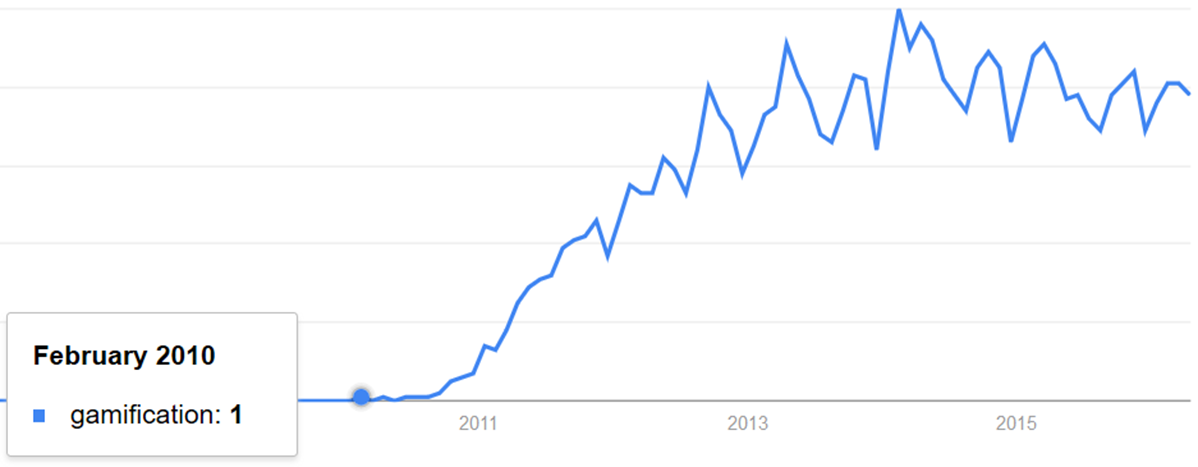
\includegraphics[width=12cm]{gamification-trend}
\caption{``Gamification" on Google Trends per 12 April 2016.}
\label{gamification-trend}
\end{figure}

Real-world examples that show the success of the gamification are Duolingo\footnote{\url{https://www.duolingo.com/
}} and Re-mission\footnote{\url{http://www.re-mission.net/}}. Duolingo is a gamified system of language learning. It embeds game elements, such as points, levels, and lives, to make language learning more fun. Re-mission is a third-person shooting game dedicated to young cancer patients and designed to teach and learn how to deal with cancer. The patients are invited to take part in an entertaining gameplay that will affect their specific behavioural and psychological outcomes producing effective cancer therapy.
 
Through a systematic review, Connolly et al. \cite{connolly2012systematic} studied the impact of computer games and serious games on engagement and learning in diverse fields. They reported the majority of the studies presented empirical evidence about the positive impact of computer games and serious games. Using the same type of method, Hamari et al. \cite{hamari2014does} found that according to the majority of the reviewed papers, gamification does generate benefits and positive effects. Specifically in the field of software engineering, Pedreira et al. \cite{Pedreira2015} also performed a systematic review on the application of gamification in software engineering. Most existing studies focus on software development, project management, requirements, and other support areas, but none of them focuses on software modelling. They also found fewer studies reporting empirical evidence to support gamification research. They argued that existing studies in the field are quite new, thus more research effort is needed to investigate the impact of gamification in software engineering. 

Reports of the positive impact of gamification in various fields encourage us to apply it in software modelling learning, an area which has received little attention for the application of gamification so far. This situation broadens our opportunity not only to produce a novel approach to teaching software modelling but also to improve gamification processes through the application of Model-Driven Engineering approaches. This research proposes a main research question, ``Can gamification improve software modelling learning?". The word `improve' implies that learning with gamification enhances learners' engagement and learning performance. The engagement of learners with the support of gamification is more durable, frequent, and active compared to learners that only use didactic approach. Also, the former perform better in knowledge and skill acquisition and application compared to the latter.   

In the beginning, we plan to address software modelling in Model-Driven Engineering as a whole---comprising modelling, metamodelling, and model transformation. However, after consideration regarding scope and time, we adjust our scoping just to focus on graphical software modelling, which is a common way to express models in modelling and metamodelling. We excluded model transformation since its approaches are commonly expressed in a textual way. We include metamodelling since a metamodel itself is a model of models and usually is expressed in the form of class diagram-like graphics. We plan to perform literature study and develop a prototype in the first year and address modelling and metamodelling in the second year and third year respectively. 
    
Instead of developing the software modelling games manually, we plan to follow a model-based approach. We will develop a design framework for the games, which will systematically and semi-automatically drive gamification design to produce software modelling learning gamification (SMLG). Essentially, our study lies in the intersection between software modelling, learning, and games as depicted in Figure \ref{smlg}. Therefore, pedagogical aspect cannot be neglected. We will apply several learning models from pedagogy to drive the design of our learning game. We also target the gamification is suitable for higher-level undergraduate and postgraduate students with some of experience of software engineering. 

The remainder of this report is organised as follows. We provide a detailed literature review in Section 2 and propose the research proposal as well as the research methodology in Section 3. Finally, in Section 4, we end this qualifying dissertation with a discussion on our preliminary results. 

\begin{figure}[ht]
\centering
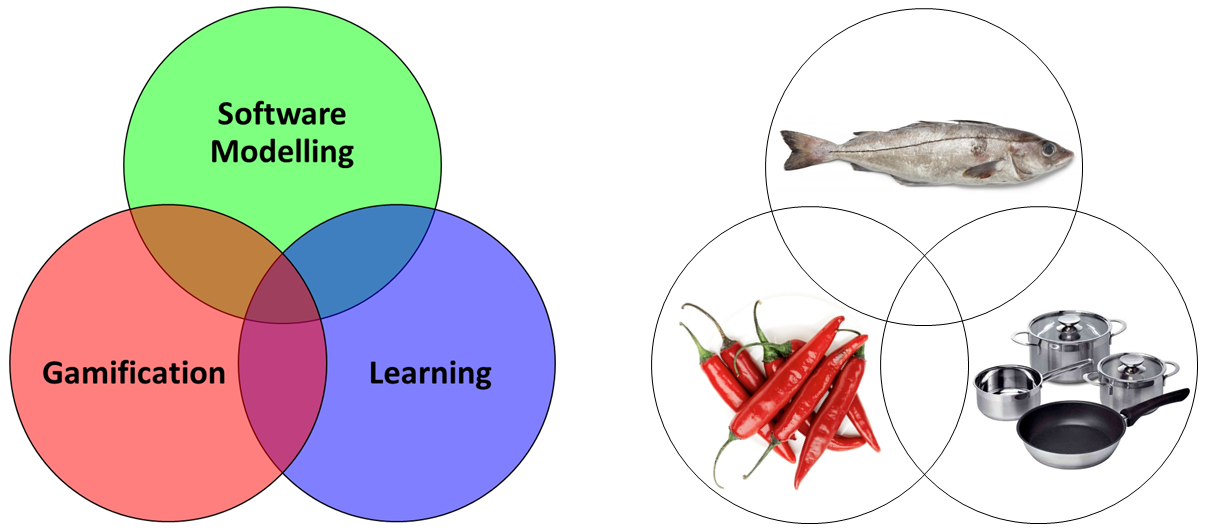
\includegraphics[width=\textwidth]{smlg}
\caption{How to 'Cook' a Gameful Software Modelling Learning?}
\label{smlg}
\end{figure}




\chapter{Field Survey and Review}
\label{Field Survey and Review}
The research underpinning the gamification of software modelling learning is multidisciplinary. Therefore, the literature review is organised by the contributing fields, including the subtopics resulting from the interaction between them. Three major contributing fields are pedagogy, ludology, and software modelling (Figure \ref{smlg2}). They are discussed below, and a brief review of the research methodology concludes this chapter.

\begin{figure}[ht]
\centering
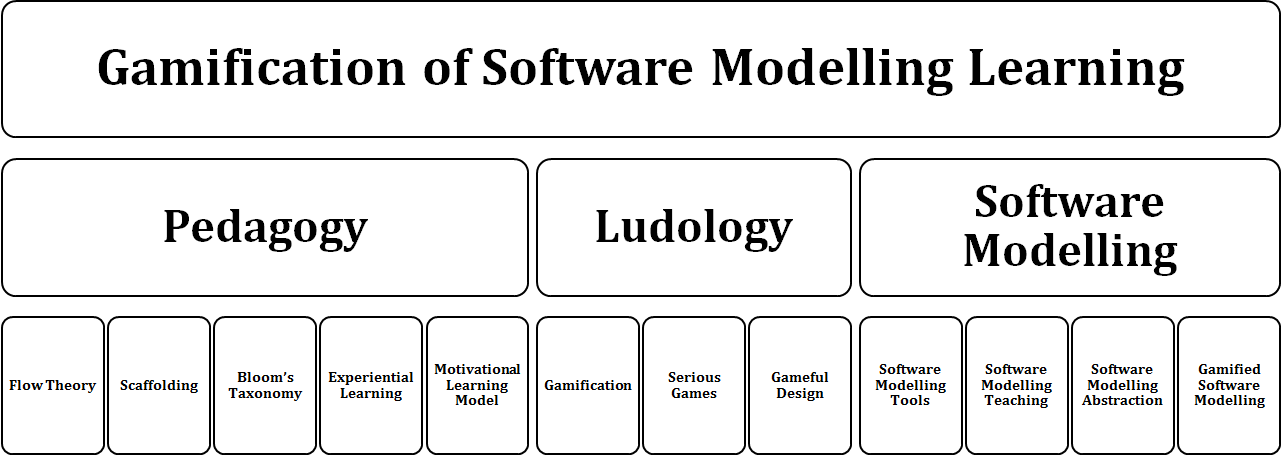
\includegraphics[width=12cm]{smlg2}
\caption{Contributing fields to the gamified software modelling learning.}
\label{smlg2}
\end{figure}

\section{Pedagogy}
\label{Pedagogy}
Designing the gamification of software modelling learning cannot be separated from the field of pedagogy since the core process supported by the gamification is a learning process. There is an abundance of literature in the field of pedagogy how we can understand learning processes and from it, we could draw principles that will guide the design of SMLG. 

We have investigated literature in the field pedagogy regarding teaching and learning. The studies that we investigated are Flemming's VARK modality model \cite{fleming2006learning}, Flow theory \cite{csikszentmihalyi2014toward}, Revised Bloom's taxonomy \cite{krathwohl2002revision}, Gardner's multiple intelligence \cite{gardner2011frames}, Felder's learning styles \cite{felder1988learning},  scaffolding \cite{wood1976role, vygotsky1978mind}, experiential learning \cite{kolb2014experiential}, self-determination theory \cite{ryan2000self}, and Keller's motivational learning model \cite{keller2010motivational}. However, we identified only five learning models that are relevant to our research since they have characteristics that we considered will address certain design concerns of our gamification. We excluded the self-determination theory from our research since one of its three components counts relatedness---one's need to get along with others---as one of the main motivations in learning, which we view is not relevant to this research. The rest are excluded since the studies focus on learning styles and preferences and why learning processes should accommodate them, which is not in line with our work that depends heavily on visual modality--extensive use of graphics for modelling. Therefore, we only discuss the selected five models in the following subsections.

\subsection{Csikszentmihalyi's Flow Theory}
Csikszentmihalyi \cite{csikszentmihalyi2014toward} proposes the theory of Flow which states that to maintain learners' engagement in an activity, the given challenges and their competence have to be kept balanced. If the challenges are too difficult, they will arrive at a state of anxiety that demotivates them and then affects them to withdraw from the activity. On the other side, if the challenges are too easy and their competence is very advanced, they will be in the state of boredom which also makes it likely for him to withdraw from the activity (Figure \ref{flow-theory}).

\begin{figure}[ht]
\centering
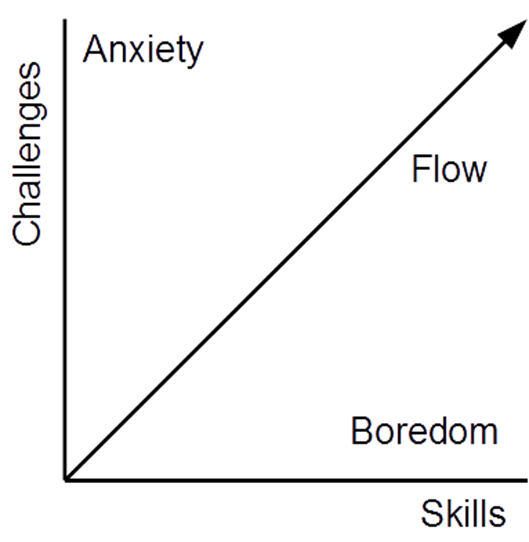
\includegraphics[width=4cm]{flow-theory}
\caption{Csikszentmihalyi's Flow Theory \cite{csikszentmihalyi2014toward}.}
\label{flow-theory}
\end{figure}
 
Flow theory has been applied in many fields, such as education, training, and games to guide maintenance of engagement. Specifically for games, flow theory influences the design of levels. The given challenges have to be adjusted, so they match the skills of players at every stage. Chen \cite{chen2007flow} comments that well-designed games should bring their players to the flow states, balanced states between challenges and skills, delivering happiness and pleasure. In the field of education, Liao \cite{liao2006flow} also applies the theory as a framework to study the emotional and cognitive responses to distance learning systems. He claims that flow theory, the cause and effect of the flow experience, also works when students use distance learning systems.

\subsection{Zone of Proximal Development/Scaffolding}
Zone of Proximal Development (ZPD) is proposed by Vygotsky in the context of adolescent development \cite{vygotsky1978mind}. Wood et al. \cite{wood1976role} use the term scaffolding to refer to the same concept in the context of learning. The theory states that during a learning process, learners have to be reinforced, particularly for knowledge or skills that are tough to learn without the support of others, to develop their competence until they can acquire the knowledge and skills on their own (Figure \ref{scaffolding}). 

\begin{figure}[ht]
\centering
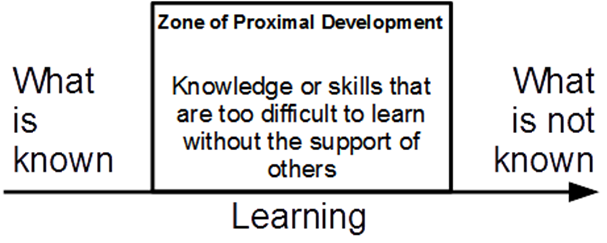
\includegraphics[width=6.5cm]{scaffolding}
\caption{Zone of Proximal Development/Scaffolding \cite{vygotsky1978mind},\cite{wood1976role}.}
\label{scaffolding}
\end{figure}

Kao et al. \cite{kao2015designing} study customised scaffolds of an educational game for learning physics, and Tsai et al. \cite{tsai2013importance} investigate the use of scaffolding aids with importance and use of targeted content knowledge in educational simulation games. Both find proper scaffolding facilitates learning and helps learners to have better performance. 

\subsection{Revised Bloom's Taxonomy}
Bloom's Taxonomy \cite{krathwohl2002revision} is a framework of cognitive levels for the learning process. The framework has been proven very useful for more than 50 years, all over the world, in supporting educators design learning processes \cite{munzenmaier2013bloom}. It consists of six activities for learners, namely remember, understand, apply, analyse, evaluate, and create, and order them according to their cognitive load levels with 'remember' at the bottom and 'create' as the activity that requires the highest cognitive load (Figure \ref{bloom}). 

\begin{figure}[ht]
\centering
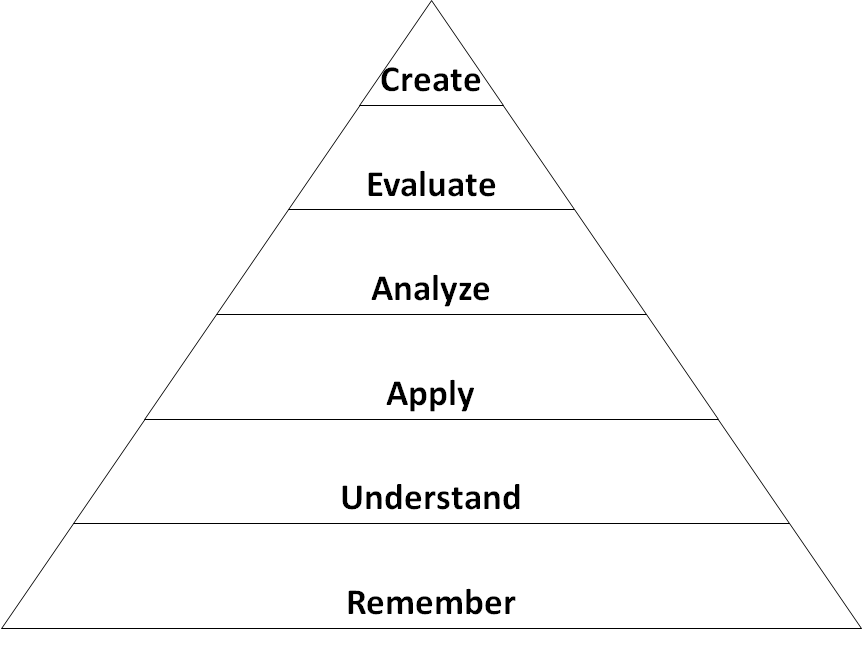
\includegraphics[width=6cm]{bloom}
\caption{Revised Bloom's Taxonomy\cite{krathwohl2002revision}.}
\label{bloom}
\end{figure}

Bloom's taxonomy has been used by other researchers in their studies. Arnab et al. utilised learning activities in the taxonomy to identify and map learning mechanics to game mechanics to construct a Learning Mechanic-Game Mechanics model for designing Serious Games \cite{arnab2015mapping}. Von Vangenheim et al. \cite{von2013scrumia} also developed an educational game for teaching SCRUM and applied activities in the taxonomy as a standard to assess the achievement of their respondents. 

\subsection{Kolb's Experiential Learning Model}
Kolb's Experiential Learning Model \cite{kolb2014experiential} is a model of teaching and learning through experience and reflection on actions. It states that knowledge development is a product of experience or iterative search. The model is a cycle consisting of four steps: abstract conceptualisation, active experimentation, concrete experience, and reflective observation (Figure \ref{kolb}). 

\begin{figure}[ht]
\centering
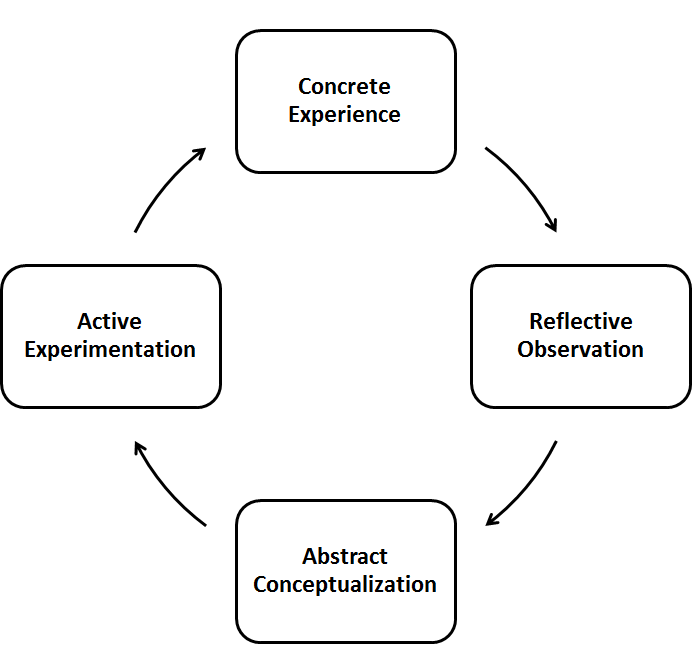
\includegraphics[width=8cm]{kolb}
\caption{Kolb's Experiential Learning Model \cite{kolb2014experiential}.}
\label{kolb}
\end{figure}

As an example, in the case of didactic learning, learners are firstly taught about the theory. In this step, learners perform abstract conceptualisation. They then move to practical activities in which they are asked to carry out some active experimentation using the theory they were taught in the class. Through experimentation, they obtain concrete experience. The results might to some degree conform to or contrast the theory. In the end, through reflective observation, the results are then reconciled with the knowledge they had acquired based on the theory, whether the knowledge is updated or not. 

A game is a potential tool to realise the experiential learning Kolb proposes, since playing games demands learners to actively participate in their course, reflect on their achievements, strategies, and outcomes, and to plan their next actions carefully to improve their performance. As showcases, Bliemel and Hassan \cite{bliemel2014game} use an IT manager-like game as an experiential learning tool and found that the experience developed during playing the game helps learners to connect IT management theories and their applications. Boctor \cite{boctor2013active} studies the use of a game that facilitates experiential learning to reinforce the learning of nursing material. His respondents found this learning method beneficial and enjoyable. 
 
\subsection{Keller's ARCS Motivational Learning Model}
Keller's Motivational Model is a set of steps for promoting and maintaining motivation in a learning process \cite{keller2010motivational}. The steps are attention, relevance, confidence, and satisfaction (Figure \ref{keller}). Attention means how to arouse learners to get their focus and awareness. Relevance uses examples and languages familiar to learners. Confidence means establishing and maintaining a positive attitude toward completing a learning process. Satisfaction is achieved when the learners' achievements are valued or rewarded. 

To maintain the motivation of learners in the process of learning, first, educators need to draw the attention of learners using a combination of novelty, surprise, aesthetics, and questions. After that, the educators should explain the relevance of the topic that is about to be explained to increase learners' motivation. To realise it, the educators could present the objectives, usefulness, instructions, motives, and contexts. Along the learning process, learners' motivation is maintained by raising the confidence of the learners through presenting their progress, performance, challenge, success, and ability. At the end of the learning process, learners should experience the satisfaction which can be realised by delivering a sense of achievement and enjoyment, as well as rewards, motivation, and feedback.

\begin{figure}[ht]
\centering
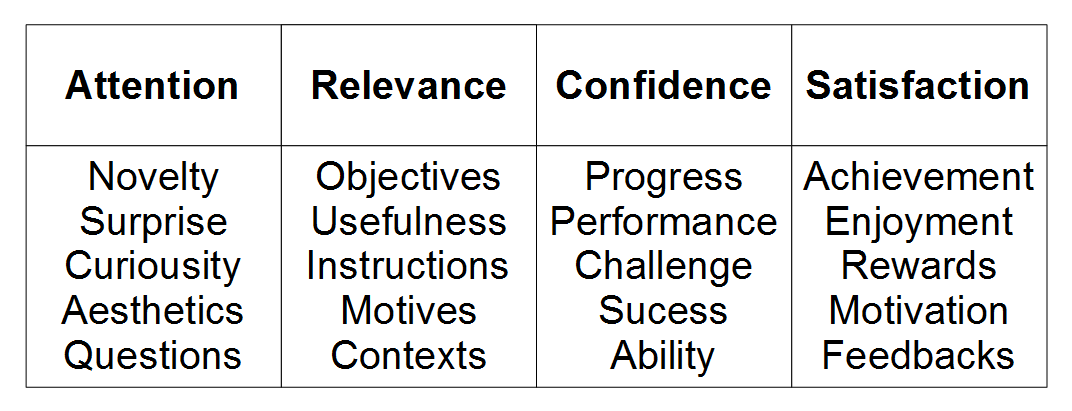
\includegraphics[width=10cm]{keller}
\caption{Keller's Motivational Model \cite{keller2010motivational}.}
\label{keller}
\end{figure}

Huang et al. \cite{huang2010sustaining} conduct an experiment using the ARCS model to examine the motivational aspect when learners play digital game-based learning and find that motivational processing (attention, relevance, and confidence) need to be considered when designing digital game-based learning. Likewise, Derbali and Frasson \cite{derbali2010players} study players' motivation while playing a serious game. Using Keller's motivational model and electroencephalography to measure learners' motivation, they identify that learning using serious game significantly increases learner motivation. 

\section{Ludology}
Ludology, the study of games, clearly is of significant relevance to our work, since it provides principles that guide the design of the gameful aspect of the SMLG. Concepts that are from Ludology, such as serious games, gamification, and gameful design framework \cite{deterding2015lens} are discussed briefly in the following sections.   

\subsection{Serious Games and Gamification}
Two terms related to games are used throughout this report: serious games and gamification. Abt \cite{abt1987serious} defines serious games ``games that have an explicit and carefully thought-out educational purpose and are not intended to be played primarily for amusement", whereas Deterding et al. \cite{deterding2011game} define gamification as ``the use of game design elements in non-game contexts". While both are used for purposes other than leisure, there is a noticeable difference. Serious games are full-fledged games---they have all characteristics to be classified as games. In contrast, gamification focuses on the use of game elements, not on a development of a complete game. 

Another confusion concerns on the word `gamification'. The word `gamification' could also be defined as a process \cite{werbach2014re}. The process adds game elements to an entity that is originally not a game, so it becomes more like a game, but there is a moment---a threshold---when we keep adding game elements, it has all the characteristics to be defined as a game---it satisfies the definition of a game \cite{yohannis2014defining}. In other words, the gamification process could transform an entity into a game, but the entity could still own its original characteristics. 

To avoid confusion throughout this report, we clarify that when we use the word `game', it could refer to two meanings. First, it relates to the common popular definition of a game, and second, it refers to the product of a gamification process. Similarly, the word `gamification' could refer to two definitions. First, it is a process---integrating game elements into an entity---and second, it is the product of the process after integrating game elements. Therefore in this report, instead of using `game' as the word that refers to the product of our gamification process, we use the word `gamification'. We use the word `game' only to refer to games that are commonly known.        

\subsection{Gameful Design Framework}
There are several existing game and gamification design-related frameworks that could be utilised to organise the integration of game elements into a learning process. Most of them are specific in a pedagogical context, but they only consider the use of full-fledged games, not game elements, in their research \cite{garris2002games, yusoff2009conceptual, de2011serious}. Others act as an inventory of problem-solution mappings where designers could choose one or more game mechanics that are appropriate to their problems \cite{arnab2015mapping, chou2013octalysis}. The rest are general procedural steps and raised from non-pedagogical contexts \cite{werbach2012win, kumar2013framework, huang2013gamification} and specifically intended for game design {\cite{hunicke2004mda}. 

However, none of the game and gamification design-related frameworks provides design guides that are relevant, reflective, innovative, and generic altogether to produce a gameful design. Relevant means gamification ideas should arise from stakeholders' needs and contexts. Reflective means a deep thinking about the interconnection between game elements and core activities that are going to be gamified. Innovative suggest that a gameful design framework should not be limited to the adoption of mechanics from a fixed inventory, but it should be stimulating enough to produce new forms of mechanics that fit with the stakeholder-specific aspects. Generic implies that the framework should be applicable in the domain of software modelling learning.

Deterding's Gameful Design framework \cite{deterding2015lens} is a framework that could facilitate our purpose.  Moreover, the framework has the following characteristics: (1) it bases its solution on target users' context (users, context, activities), (2) it focuses on the core activity that needs to be gamified, (3) it is concerned with the challenges and motivation that are inherent to the core activity, (4) it provokes ideation of a genuine gameful design, not just limited to a collection of game elements (game elements are used as a starting point to stimulate ideation), (5) it supports iterative prototyping, (6) it is generic and applicable across domains.               

The Gameful Design framework consists of design lenses, skill atoms, and prescriptive guidelines \cite{deterding2015lens}. A design lens is a combination of an easy-to-remember name, a brief explanation of a design principle, and questions that help designers to view activities, motivation, and challenges from the perspective of game design principle that the lens represents. Deterding's Design Lenses \cite{deterding2015lens} come with four categories of lenses: challenge, goal and motivation, action and object, and feedback. Each category comes with lenses to reflect on the activities, motivation, and challenges from game element perspective to generate innovative ideas of gamification (Figure \ref{lenses}). 

\begin{figure}[ht]
\centering
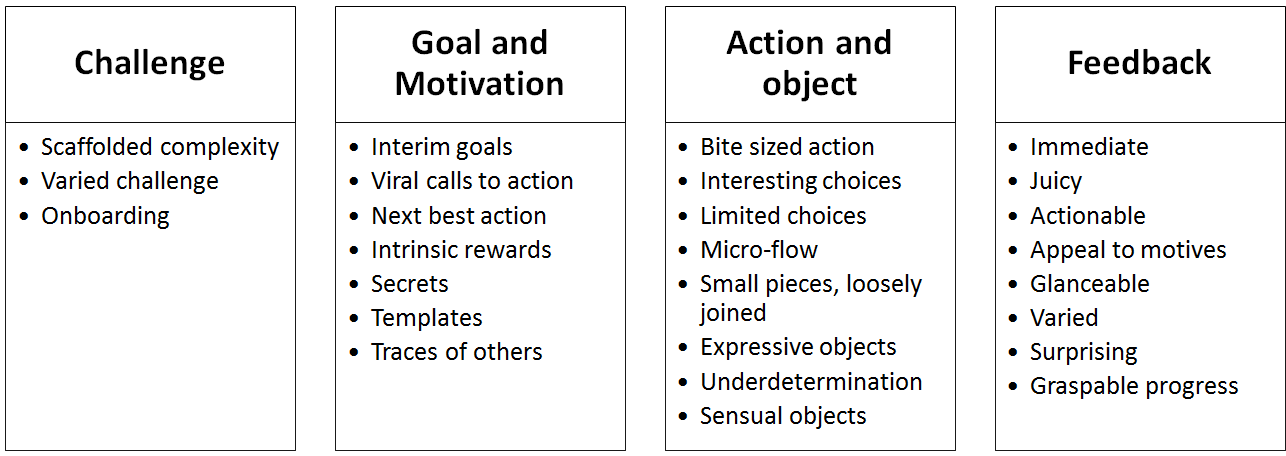
\includegraphics[width=14cm]{lenses}
\caption{Deterding's design lenses \cite{deterding2015lens}.}
\label{lenses}
\end{figure}

A skill atom describes a feedback loop between a user and that is organised around a central challenge or skill (Figure \ref{skill-atoms}). At first, the user takes actions driven by his motivations and goals, which forms inputs to the system's rule engine that determines changes of states of the system. The system then returns feedback to the user, which will be integrated into the user's mental model of the system. Through repeated action-feedback interaction, the user masters the intended skill.

\begin{figure}[ht]
\centering
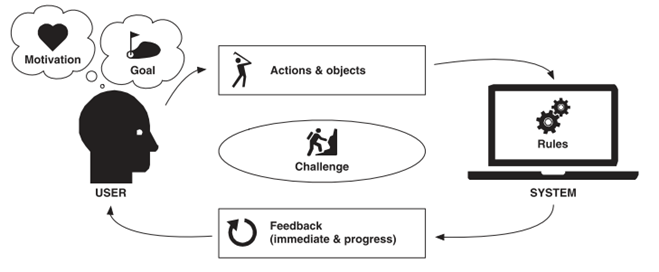
\includegraphics[width=14cm]{skill-atoms}
\caption{Deterding's skill atoms \cite{deterding2015lens}.}
\label{skill-atoms}
\end{figure}

The prescriptive guidelines of the Gameful Design framework comprise five phases: strategy, research, synthesis, ideation, and iterative prototyping. In the strategy phase, stakeholders define outcome metrics, target users, context, and activities as well as constraints and requirements. In the next phase, the research phase, user activity, behaviour chains, user needs, motivations, and challenges are identified and defined. After that, in the synthesis phase, activity-challenge-motivation triplets are defined, including defining skill atoms. Next, in the ideation phase, ideas are generated for the gamification design, brainstorming with innovation stems is conducted and design lenses are used to help determine appropriate game elements that fit with the triplets. After some ideas are generated, those ideas are prioritised and translated into storyboards to make them more visible. After that, the ideas are evaluated and refined based on results of the evaluation. In the last phase, a prototype is developed iteratively, including the activities of playtesting, analysing, building, and generating new ideas. 

\begin{figure}[ht]
\centering
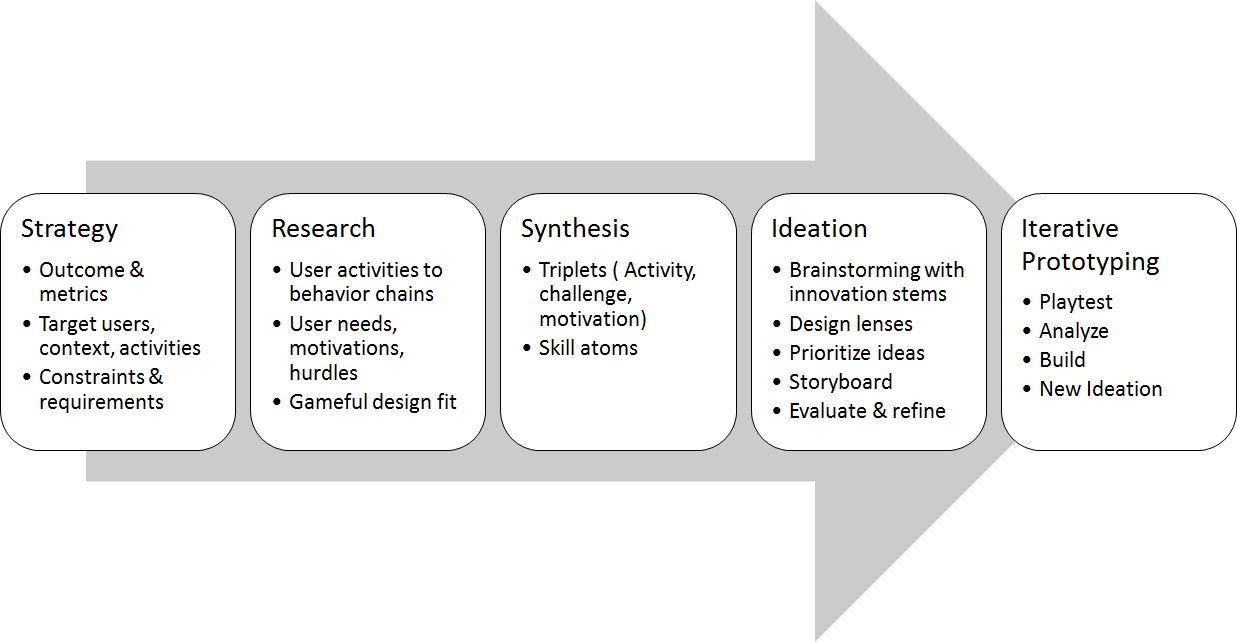
\includegraphics[width=14cm]{gameful-steps}
\caption{Deterding's gameful design steps \cite{deterding2015lens}.}
\label{fig:gameful-steps}
\end{figure}


\section{Software Modelling}
While pedagogy provides methods for delivering learning contents and ludology contributes to improving the motivation in a learning process, software modelling is the actual learning topic that this research is concerned with. In this section, we discuss what software modelling is, tools to perform software modelling, existing principles and practices in software modelling teaching, abstraction in software modelling and related studies of gamified software modelling.    

\subsection{What is Software Modelling?}
Software modelling creates abstract models of domains to explore and manage the development of software typically using less-abstract-models that target a particular software manifest. Modelling has a crucial role in Model Driven Engineering (MDE) methodology since MDE harnesses greatly the strength of modelling to improve engineering processes \cite{brambilla2012model}.  

\begin{figure}[!b]
\centering
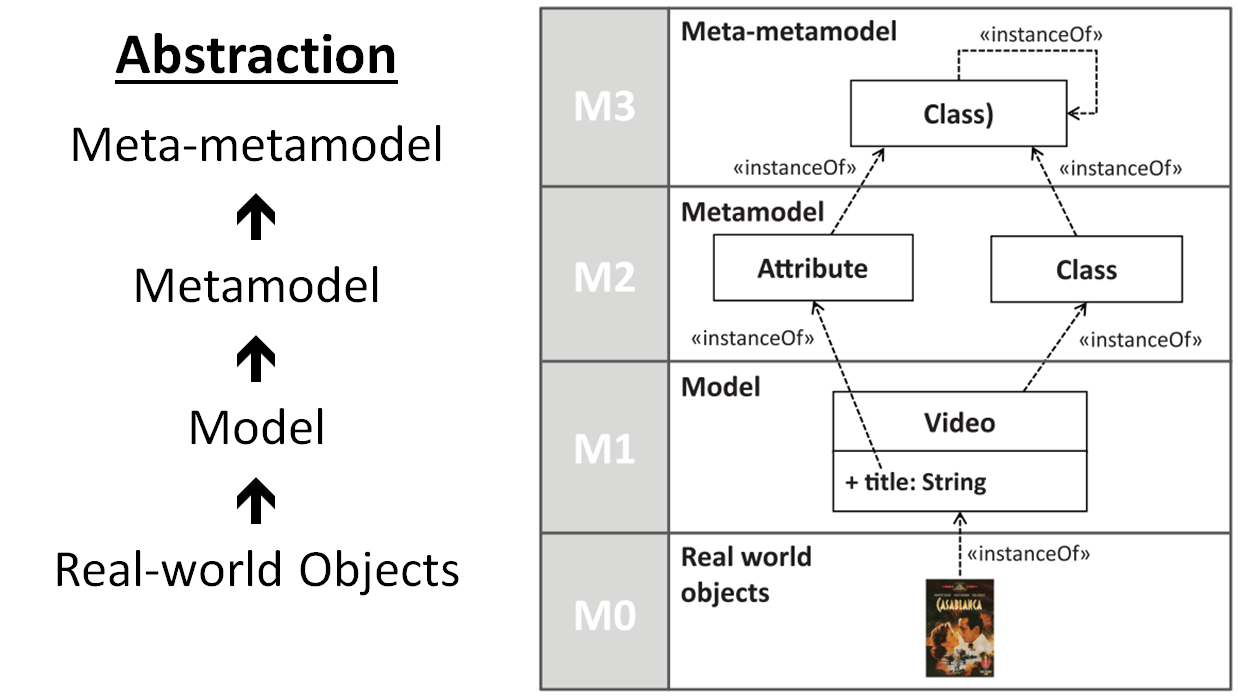
\includegraphics[width=13cm]{abstraction}
\caption{Abstraction in Model-driven Engineering \cite{brambilla2012model}.}
\label{abstraction}
\end{figure}

The process of modelling itself often starts from real world objects---a concrete experience---and then applies a process of abstraction \cite{white2010teaching, engels2005teaching}. Typical modelling architectures have four layers. The first layer is real world object, the second layer is the model, the third one is the metamodel that defines the language of the model, and the fourth one is the metametamodel \cite{brambilla2012model}. Models are abstractions of real-world objects. Models can also be abstracted in the form of metamodels, models that describe models. Likewise, the metamodels can be abstracted further in the form of metametamodels, models that define metamodels. In practice, metemetamodels can be defined regarding themselves, to remain within four levels of abstraction, rather than creating infinite levels of modelling. This process of abstraction is depicted in Figure \ref{abstraction}.
 
To create real working systems, models have to be transformed into software. We call this whole process as concretisation, a process that has a reverse direction to abstraction. Figure \ref{concretisation} illustrates a process of conretisation of a metamodel of a flowchart language used to the waking-up process. The metamodel constitutes the definition of a language that defines the model since it has rules to describe the model represented by the language \cite{brambilla2012model}. So, every model created should conform to its metamodel. The metamodel is more general than it is models since it could be applied to different model domain. In Figure \ref{concretisation}, the metamodel is instantiated to model the process of waking up. Through model transformation and instance generation, the model is taken as an input to generate a working system, in this example, a simple algorithm for waking up and turning off an alarm.   

\begin{figure}[!t]
\centering
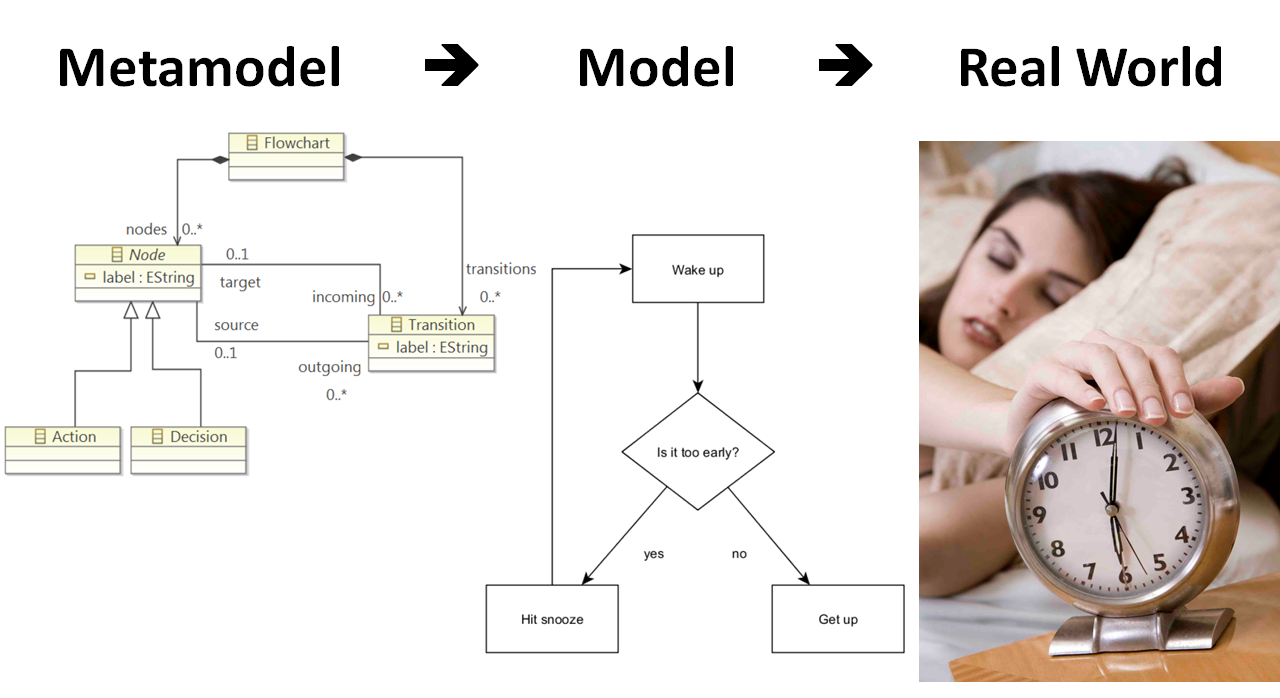
\includegraphics[width=13cm]{concretisation}
\caption{Instantiation in Model-driven Engineering.}
\label{concretisation}
\end{figure}
   
\subsection{Software Modelling Tools}
The use of tools for software modelling is encouraged since with them we can easily manipulate models, create models that at least conform to their metamodels, and perform model transformation \cite{brambilla2012model}. There are many tools available for software modelling, ranging from general-purpose drawing tools like Dia\footnote{\url{http://dia-installer.de/}} to language-specific modelling tools like Papyrus\footnote{\url{https://eclipse.org/papyrus/}} and from  simple modelling tools for learning \cite{dranidis2015learning} to enterprise-scale modelling suites \footnote{\url{https://www.visual-paradigm.com/features/}}. 

\begin{figure}[!ht]
\centering
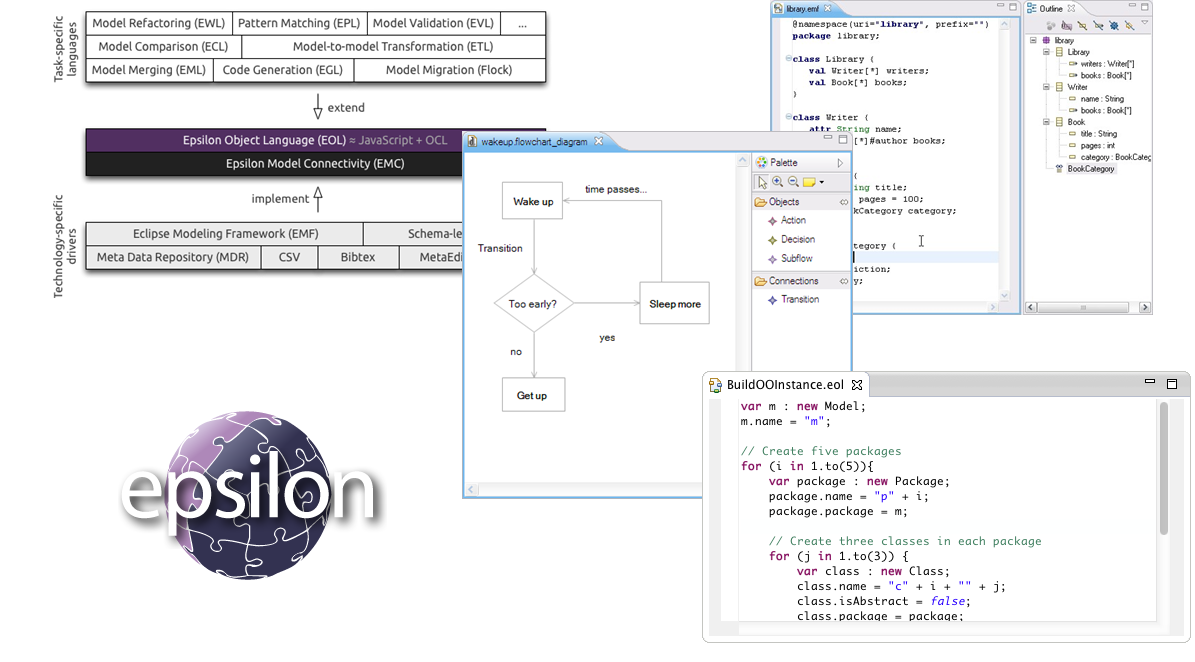
\includegraphics[width=\textwidth]{epsilon}
\caption{Epsilon is a family of languages and tools for model management \cite{kolovos2010epsilon}.}
\label{epsilon}
\end{figure}

For the purpose of learning, Dranidis et al. \cite{dranidis2015learning} and Akayama et al. \cite{Akayama2013} suggest developing simplified software modelling learning tools, since, for beginners, modelling using professional tools can be overwhelming. Once learners master the fundamentals of software modelling, they can move to more advanced topics, such as metamodelling and model transformation. One tool that supports advance model operations is Epsilon. Epsilon is a family of languages and tools for model management \cite{kolovos2010epsilon}. The model management itself consists of several processes. They are code generation, model-to-model transformation as well as model validation, comparison, migration and refactoring. Moreover, Epsilon also supports Eclipse Modeling Framework (EMF) and other model types, such Meta Data Repository (MDR), CSV, Bibtex, etc. (Figure \ref{epsilon}). Epsilon also has an extension called EuGENia which is dedicated to producing graphical modelling editors automatically\cite{kolovos2015eugenia}.

\subsection{Software Modelling Teaching}
\label{Software Modelling Teaching}
We have investigated related literature regarding the teaching and learning of software modelling. From the literature, we have identified findings and categorised them into three groups: contents, teaching or learning practices, and tool design. The findings are to be considered as requirements for the design of gamification of software modelling learning. 

\subsubsection{Contents}
Contents mean the software modelling topics and their structures. In teaching software modelling, we need to teach the core, important concepts and their relation with the contexts and applications of the outside world. The contents of software modelling learning should address software modelling definition at first \cite{borstler2012teaching} and then teach modelling foundation, such as semantics, syntaxes, and notation \cite{borstler2012teaching}. However, the teaching should focus on semantics, not only syntax \cite{borstler2012teaching}, and improving the use of language, not just vocabulary \cite{bezivin2009teaching}. 

The core, important concepts of Model Driven Engineering---modelling, metamodelling, and model transformation---should be taught. Teaching modelling should comprise the following topics: formal and informal models, partial and complete models, and the distinction between models and programs \cite{bezivin2009teaching}. Nevertheless, metamodelling should be given a larger portion than modelling since a model might conform to more than one metamodel \cite{ober2007teaching}. 

Software modelling is an engineering subject. Therefore, we should teach the engineering aspects of software modelling, such as understanding a domain, planning and resourcing, documentation, quality, formality, validity, and optimisation \cite{paige2014bad}.

Another important topic in teaching software modelling is the practices or applications of software modelling in various domains \cite{ borstler2012teaching, paige2014bad}, including their success stories, code generations, model discovery, and model-driven interoperability. It's best to make model executable, since the power of execution makes it much easier to understand the model \cite{bezivin2009teaching}.

\subsubsection{Teaching and Learning Practices}
Through our literature review, we identify some teaching and learning practices of software modelling suggested by experts based on their experience teaching software modelling. The practices are discussed in the following paragraphs.

Modelling is a process to think abstractly about systems. Therefore, modelling is thaught to make students understand the value of abstraction \cite{bezivin2009teaching}. Additionally, successful application of Model-Driven Software Development depends on abstract modelling skills \cite{whittle2013industrial}. Another best practice suggested is that software modelling should be taught with prerequisites \cite{paige2014bad}. Therefore, the learners should have a good programming background \cite{bezivin2009teaching} or know a little about OOP \cite{Akayama2013}. However, for an introduction to modelling in computer science/software engineering programmes, we can teach modelling alongside with programming\cite{borstler2012teaching, bezivin2009teaching}. In this way, students can learn to model as early as possible \cite{Akayama2013, borstler2012teaching}. 

In teaching software modelling, we should encourage students to produce ``good" models and measure their ``quality", therefore they will be informed how good are their models. One way to measure the quality of models is using tools \cite{Akayama2013}. In teaching software modelling, problem-solving should be taught first, while modelling language specification and modelling tools can get in the way \cite{paige2014bad}. Regarding the problem-solving approach, educators should give solutions, not just direct answers \cite{paige2014bad}. Another best practice is that educators should teach modelling language broadly, not deeply \cite{paige2014bad}, and throughout \cite{borstler2012teaching}. Students need to experience the whole cycle of modelling in a software engineering project, so they learn to decide which development process is more appropriate than the others \cite{Akayama2013}. Consequently, teaching should refer to other disciplines or other aspects related to software modelling as well \cite{paige2014bad}.

Even though code generation is essential to understand modelling, since it shows the real-world application of Model-Driven Engineering, educators need to teach other applications (benefits) of software modelling at first \cite{liebel2015ready}. The code generation could come later \cite{paige2014bad}. Also, the educators should be careful when using analogies and physical decomposition since they might not reflect the complexity of the system; one component might have a cross-cutting effect to other layers of the system \cite{paige2014bad}. Furthermore, it is good to teach modelling with a standard language, such as UML \cite{bezivin2009teaching}. However, educators need to teach modelling and meta-modelling using other modelling languages as well, not just UML. Software modelling is not a UML modelling course \cite{paige2014bad}. A significant number of successful Model-driven Software Development companies build their own modelling languages and generators, suggesting a re-orientation of education away from UML notation to fundamental modelling principles \cite{whittle2013industrial}. Choosing a playful domain or fun problems, not serious domain, is suggested to increase learners' engagement \cite{paige2014bad}.

\subsubsection{Tool Design}
Tool design is the principles for designing software modelling tools. Since we are going to develop a tool that can support learners to learn software modelling, lessons in this category are important in guiding the design of our tool. 

We can teach software modelling using papers, tools designed for pedagogy, or mainstream tools \cite{Akayama2013}. Each comes with its advantages and drawbacks. For an introduction, paper is a good choice. The use of modelling tools is not important in the beginning, but later when the modelling task becomes larger, more advanced tools could be considered \cite{bezivin2009teaching}. However, learning modelling tools is not trivial \cite{paige2014bad}. Considerable efforts required to become fluent using a tool. A good experience with a tool has a positive influence on learners' view on modelling \cite{liebel2015ready}. Likewise, support for tool usage also affects student satisfaction greatly. So, if industry modelling tools are used, it is critical to provide adequate support, such as providing access to a tool expert and carefully designing the instructions \cite{liebel2015ready}. For example, Papyrus is suitable for a classroom environment if it is given with the right level of support \cite{liebel2015ready}.

Based on his experience developing an educational software modelling tool, Lethbridge \cite{lethbridge2014teaching} proposed the following best practices to produce a good educational modelling tool: (1) build knowledge and skills incrementally, (2) give positive reinforcement to learners, (3) the tools offer maximum opportunities for learning, (4) the tool convinces learners of the value of what they learn, (5) focus on high usability, and (6) the tool is inexpensive.

\subsection{Abstraction in Software Modelling Learning}
\label{Abstraction in Software Modelling Learning}
The review of software modelling and its teaching leads us to conclude that modelling and meta-modelling, and additionally model management, are potential concepts to be taught in the game. All three concepts require adequate abstraction skill, a skill that we have shown to have a fundamental role in computer science and software engineering \cite{engels2005teaching, Kramer2007, hazzan2008reflections}. There are some available strategies for teaching abstraction. One of them is the Familiarity, Similarity, Reification, and Application steps proposed by White and Mitchelmore \cite{white2010teaching} for mathematics. They argue that abstraction should be developed from empirical experience to abstraction. The abstraction then is reified to become an application. Similarly, based on their experience teaching UML, Engels et al. \cite{engels2005teaching} approach abstraction through modelling following three steps: real-world objects, object diagrams, class diagrams. The real-world objects can be described by videos or may be substituted by textual explanation, animations, or pictures. Hazzan \cite{hazzan2008reflections} proposes three methods in teaching abstraction. First, illustrate: the lecturer uses abstraction-related words or statements in teaching. Second, reflect: for example, the lecturer and students question the impact of using a certain level of abstraction or not using abstraction at all. Third, practice: students must practice and reflect on the use of abstraction. 

There are two approaches to learning software modelling which learners may perform simultaneously: a rational approach and an intuitive approach \cite{bobkowska2014software}. Usually, at the beginning of the modelling process, learners use their existing knowledge and logical reasoning to understand and develop software models, sometimes preceded by empirical activities. However, there are situations in software modelling where existing knowledge and methodology-based, logical reasoning are not enough to allow learners to understand or to develop a software model. In this situations, the learning might expect the learners to rely on their intuition, might present a combination of both rational and intuitive approaches. Moreover, in building a model at an appropriate level of abstraction, one needs a level of intuition and skill which cannot be gained through lectures alone, but has to be experienced through exercises \cite{engels2005teaching}. This approach is also encouraged by experiential learning \cite{kolb2014experiential}.   

\subsection{Gamified Software Modelling}
\label{Gamified Software Modelling}
Most of the gamification studies available related to software engineering in a wider context or other aspects of software engineering, such as software implementation and project management, rather than software modelling in particular \cite{Pedreira2015}. Studies that apply gamification specifically for software modelling include Stikkolorum et al. \cite{Stikkolorum2014}, Ionita et al. \cite{Ionita2015}, Groenewegen et al. \cite{Groenewegen2010}, and Richardsen \cite{Richardsen2014}. findings from these related studies are presented in section \ref{Research and Design Implication}.

\subsubsection{Puzzle Game to Teach Software Design Principles}
Stikkolorum et al. \cite{Stikkolorum2014} develop a game that is intended to teach software design principles, such as cohesion, coupling, information hiding, and modularity in object-oriented software design. They look for a solution that provides a balance between coupling and cohesion by using a toolbox to draw classes, methods, attributes, and relationships. They apply game elements like puzzles, game levels, visual and audio feedback, a progress indicator, level unlocking, choice of paths, multiple solutions, and scoring. For the pedagogical aspect, they refer Bloom's taxonomy in their work. However, they did not explain how they integrated the taxonomy into their work. They validate their design by conducting user test and utilised the 'think aloud' method, asking users to tell their thoughts while using the game. After using their game, Stikkolorum et al. \cite{Stikkolorum2014} observe that users start to refer to concepts such as classes, methods, and associations instead of boxes, blocks, and lines, indicating a progress of learning. The main challenge of their work is related to scoring since there are many valid solutions for a problem. To determine coupling, they use the Coupling Between Object Classes (CBO) metric \cite{Stikkolorum2014}. Cohesion was measured by comparing all items---attributes, methods, class name---that have similar keywords under the same class. Information hiding and modularity is evaluated using general design patterns. 


\subsubsection{Explorable Board-game to Understand and Validate Enterprise Architecture}
Groenewegen et al. \cite{Groenewegen2010} apply gamification to improve stakeholders' understanding of their enterprise architecture models as well as to validate them. They employ board game-like technique---exploring model step by step, element by element according to the given rules---which can provide a player with a progressive user experience. Therefore, it can improve user understanding. The game proposed is more playable than before, more freedom to try and explore, and no explicit rewards were given. For the game elements, they utilise cards, explorable board-game, and rules. They claim that users can understand the model better than by merely looking at it, so they can argue whether the model is valid or not based on their existing knowledge. However, they do not give any pedagogical reason of the claim. The challenge that they experience during the implementation is translating modeller's and reader's implicit knowledge unto explicit knowledge in the model---a gap of knowledge between the modeller and the reader, which domain knowledge is required. Lack of domain knowledge makes a model less understandable, and users cannot validate the model. For validation, they test their work to seven respondents and then interviewing them. 

\subsubsection{Familiar Tangible Model to Model Information Security}
In the domain of information security modelling, Ionita et al.\cite{Ionita2015} develop a socio-technical modelling language (TREsPASS) that maps information on security-related concepts toward tangible representation. Mapping the socio-technical modelling language to the tangible model, a model that uses physical objects as representation of concepts, is the most challenging part of their work. The tangible representations are claimed to increase the familiarity and understandability of models, which could raise awareness, involvement, and learnability. For the game elements, they utilise familiar, tangible representations, such as Lego characters, a board-game metaphor, and rules. The paper discusses the pedagogical aspect of their design which is based on constructivism, cognitive load, and cognitive fit. Moreover, based on their experiment, they reported that an experimental group performed better than a control group in learning, efficiency, correctness, and satisfaction. Likewise, based on an interview with experts and professionals, the respondents argued that the tangible model might be useful for less technical domain experts and different types of stakeholders to be more participative and contributive in the early stages of architecture modelling.

\subsubsection{Arranging UML Activity Diagrams to Control the Behavior of a Game}
In the context of activity diagram learning, Richardsen \cite{Richardsen2014} develops a game, whose behaviours are controlled through an UML activity diagram. Throughout his research, he identifies a challenge in controlling the game from the activity diagram in the Reactive Block Environment\footnote{\url{http://reference.bitreactive.com/}}, an eclipse-based visual development environment for Java application that is difficult since Eclipse\footnote{\url{http://www.eclipse.org/home/index.php}} is difficult for a first-time user. For validation, he conducts user testing with three users. The `think-aloud' method is used for observation. After that, questionnaires are given, and an interview is conducted. He concludes that there is no significant difference between the traditional interactive tutorial and the game-like tutorial on their performances. However, the game-like tutorial is more engaging. For the validation of his work, the author does not mention any explicit pedagogical aspects.\\

\section{Research and Design Implication}
\label{Research and Design Implication}
So far, we have presented studies categorised in pedagogy, ludology, and software modelling fields. In this subsection, we summarise the related studies and present findings and the plan briefly for how we are going to integrate the findings into our research.     

\textbf{Pedagogy}. In the pedagogy domain, we have presented learning models that we plan to apply in our design, including the theory of Flow, Scaffolding, Bloom's taxonomy, experiential learning, and motivational learning. Each model has its contributions to the design of our game. Theory of Flow tells us that in order to maintain learners' motivation, their competence and given challenges have to be kept balanced \cite{csikszentmihalyi2014toward}. We plan to use the theory to guide the design of levels, balancing challenges and learners' competencies. Scaffolding suggests us to give reinforcement to learners to help them grasp difficult but important concepts \cite{wood1976role, vygotsky1978mind}. We plan that our gamification should also provide scaffolding to learners. It should present helpers and cues to learners to help them solve problems and grasp key concepts. The scaffolding will be removed gradually as the competence of the learners grows. 

Moreover, Bloom's taxonomy provides us six activities with different cognitive loads \cite{krathwohl2002revision}. We see the potential of the six activities of Bloom's taxonomy: the activities that the learners will perform when playing the gamification and the nature of cognitive load of each activity could be applied to the challenges of each level. Thus, Bloom's Taxonomy will give us a variety of options---activities and challenges---in designing the levels of our game. Kolb's model gives us a framework to design a learning activity cycle for experiential learning \cite{kolb2014experiential}. We plan to apply the model to the design of our gamification so it will allow learners to perform active experimentation and develop their understanding of software modelling and make connection between their knowledge and real experiences. The motivational model provides us four components that we should consider to maintain learners' motivation \cite{keller2010motivational}. The model to be applied to the design of flow of a level of a SMLG to maintain learners' motivation. We will elaborate and discuss these learning models and our design in more detail in section \ref{Elaborating Design and Learning Models}. 

\textbf{Ludology}. In this report, we will use the term `gamification' to represent games or products that are the target results of gamification processes. To guide our gamification design, we choose Gameful Design framework \cite{deterding2015lens}, since we judge the framework stimulates innovative gamification ideas arose from stakeholders' needs and contexts through a deep thinking about the interconnection between game elements and core activities that are going to be gamified. Up to now, we have followed the prescriptive guidelines of the Gameful Design framework to generate the preliminary design of our game and developed a storyboard to create a visual representation of our design (Appendix \ref{Storyboards}). We also have performed our preliminary survey to identify learners' needs, motivations, and challenges (section \ref{Preliminary Survey}). The result of our initial design and its early prototype can be found in section \ref{Game Design}.

\textbf{Software Modelling}. In sections \ref{Abstraction in Software Modelling Learning} and \ref{Software Modelling Teaching}, we have investigated studies related to abstraction in learning, specifically in software modelling, and best practices in teaching software modelling. From these related studies, we derive several design requirements, which can be found in section \ref{Design Requirements}. From gamified software modelling related studies in section \ref{Gamified Software Modelling}, each study addresses different topics in software modelling. However, none of them addresses the core topics of Model-Driven Engineering---modelling, meta-modelling, and model transformation, which means that there is an opportunity for novel research in the area. We also found that each study addressed its topic with different approaches and game elements, which also challenges us to develop a more generic design in addressing software modelling learning problems. Moreover, the common drawbacks of the studies are that most of them did not consider the pedagogical aspect of their solution and their validation was weak in sample size as well as the lack of discussion of internal validity. Nevertheless, all of the studies reported that their gamified approaches have a positive effect---it is motivating and engaging users in varying degrees, which confirms that gamification has a positive impact on motivation.

Still from gamified software modelling related studies in section \ref{Gamified Software Modelling}, we also identified some constructive findings to improve the quality of our research and gamification design. First, the quality of models created by learners has to be measured to give them feedback how good the models are. Software metrics could be applied to measure the quality. Second, evaluation should conform to the standard criteria of good research practices in terms of sample size and internal validity. Third, pedagogical aspect should be integrated into gamification design.       

\textbf{Output Tool and Framework}. Simplified software modelling learning tools for learning purpose are appropriate for beginners since modelling using professional tools can be overwhelming \cite{dranidis2015learning, Akayama2013}. Thus, we plan to build our gamified modelling tool, a tool that is simple, familiar, and accessible. Simple means the tool focuses on core activities so learners can easily learn software modelling. Focusing on core activities also satisfies the requirement of gameful design \cite{deterding2015lens}. Familiar means the tool mimics common visual modelling environments that usually take in the form of a window that has a palette and a drawing area. Accessible means the tool is a web-based application so learners can access the tool as long as they have an internet connection.

We also plan to build a design framework for SMLG to ease the design of gamification and automate the generation of the learning gamification. The design framework will be built upon the Epsilon family, including the utilisation of other technologies such as Javascript, HTML, and J2EE to create web-based learning gamification. Epsilon is a family of languages and tools for model management \cite{kolovos2010epsilon}. The model management itself consists of several processes. They are code generation, model-to-model transformation as well as model validation, comparison, migration and refactoring. Moreover, Epsilon also supports Eclipse Modeling Framework (EMF) and other model types, such as Meta Data Repository (MDR), CSV, Bibtex, etc. (Figure \ref{epsilon}). A visual modelling environment for the design framework will be generated using EuGENia \cite{kolovos2015eugenia}, a subset of Epsilon family intended to produce visual modelling editors automatically.

\chapter{Proposal}
\label{Proposal}
Grounded on the literature review in Chapter \ref{Field Survey and Review}, in this section, we present our research questions as well as our research aim and objectives to answer the questions. We also present the possible research outputs that will be produced by our research and the research methodology that we are going to apply to address the research questions.   

\section{Research Questions}
The main research question proposed by this research is ``Can gamification improve software modelling learning?". The word `improve' implies that learning with gamification enhances learners' engagement and learning performance. Learners with the support of gamification engage more durable, frequent, and active compared to learners that only use didactic approach. Also, the former ones perform better in knowledge and skill acquisition and application compared to the latter ones. To answer the main research question, following sub research questions need to be investigated:
\begin{enumerate}
\item Which parts of software modelling teaching and learning could benefit from gamification?
\item What teaching and learning best practices of software modelling that are significant to be accommodated in SMLG?
\item What pedagogical learning models and in what roles that can improve the engagement and effectiveness of SMLG?
\item What kind of gamification design that can support software modelling learning best? 
\item What kind of orchestrating framework is needed to design the interaction between software modelling and game elements to achieve effective software modelling gamification?
\item To what extent does gamification of software modelling improve learners' motivation, engagement, and performance?
\item To what extent do software modelling tutors benefit from a software modelling game design framework?
\end{enumerate}

\section{Objectives}
\label{Objectives}
The main aim of this research is to assess to what extent gamification can improve software modelling learning. Therefore, we will investigate and develop a software modelling game design framework that systematically and semi-automatically drives gamification design to produce SMLG. More precisely, this research aims to meet the following research objectives that are derived from the main research aim:

\begin{enumerate}
\item Perform a literature review to identify research problems, questions, and objectives. 
\item Develop a framework that is intended to design and generate gamification of software modelling learning based on the literature review and survey. The framework will be iteratively updated according to the results obtained from experiments. 
\item Design and generate instances of gamification of software modelling learning. The instances will be tested to respondents for evaluation and to obtain feedback for iterative improvement. 
\item Perform controlled experiments to measure the significance of the SMLG in improving learning performance compared to traditional method, didactic learning without the support of the gamification.
\item Perform controlled experiments to measure the productivity and maintainability of a software modelling learning design framework in supporting tutors design and develop gamified software modelling learning. 
\end{enumerate}

\section{Research Outputs}
The potential research outputs of this research are:
\begin{enumerate}
\item Artefact. Software/applications of gamification of software modelling learning. The applications of gamification are designed and generated using a gamification design framework. 
\item Modelling Artefact. A gamification design framework for modelling and generating applications of SMLG.
\item Significance. Controlled experiments, a learning outcome comparison between gamified version and the traditional one of software modelling learning.
\item Understanding. A model that explains how gamification of software modelling learning works. The model can be achieved through Learning and Game Analytics and Structural Equation Modelling studies.
\item Case Studies. Reports of applications of theories, models, and methods used in this research.
\end{enumerate}

\section{Research Methodology}
In this section, we discuss briefly the research methodology that we apply to address research questions presented previously. Since the main outputs are design artefacts---the applications of gamification and the framework to generate them, Design Science Research Methodology \cite{peffers2007design} is selected as the research method as it provides a comprehensive conceptual framework and activity guidelines for understanding, developing, executing, and evaluating the design artefact. We also discuss briefly our evaluation plan to evaluate our research findings. In the end of this section, we present our Research Data Management approach as part of good research practices.   

\subsection{Design Science Research Methodology}
We will employ Design Science Research Methodology \cite{peffers2007design} as the methodology to carry out the research. DSRM is selected since it provides a comprehensive conceptual framework that consists of activity guidelines for understanding, developing, executing, and evaluating design artefacts (Figure \ref{dsrm}). Another reason is that it positions itself at the top level of abstraction without going into much detail of how to perform each activity, we can freely choose other more concrete research methods to carry out the activities. For examples, we can conduct literature reviews, surveys, or expert interviews to determine research problems, motivations, solutions, and objectives as well as controlled experiments to measure and evaluate the effectiveness of the artefacts. 

\begin{figure}[ht]
\centering
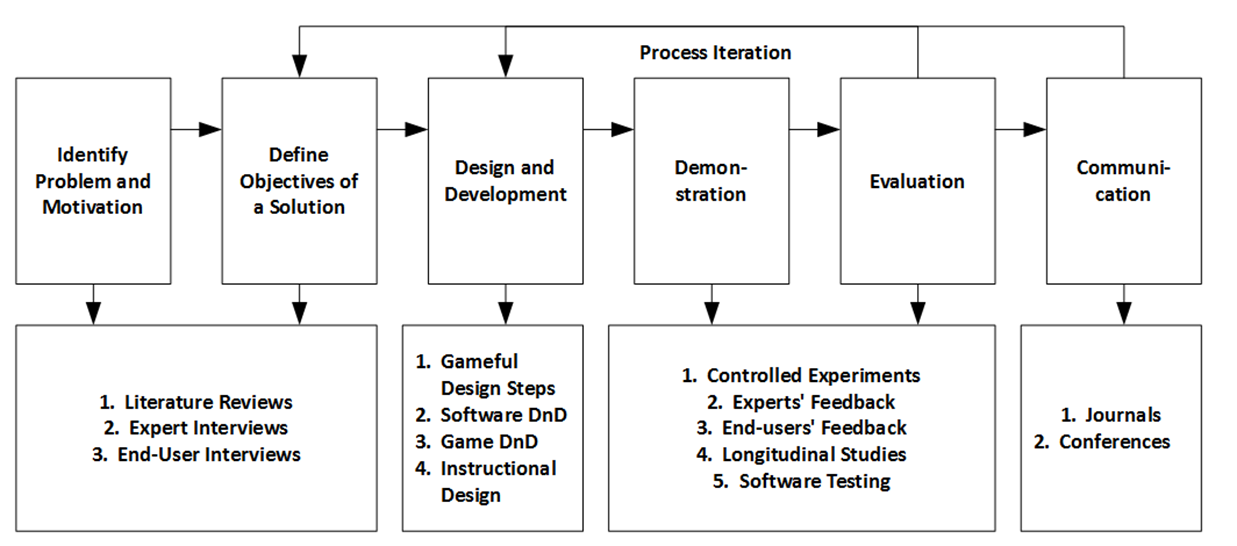
\includegraphics[width=\textwidth]{dsrm}
\caption{Design Science Research Methodology. Adapted from Peffer et al. \cite{peffers2007design}.}
\label{dsrm}
\end{figure}

\textbf{Identify Problem and Motivation}. This research will use literature review, suggestions from experts, and surveys to identify research problems and motivations as the background to determine the solution and its objectives. The experts are academicians or practitioners that have significant experience in Model-Driven Engineering and respondents are the students of Model-Driven Engineering-like modules (Software Analysis and Design, Model-Driven Software Development, etc.). In this way, (1) we can identify parts of software modelling teaching and learning that could benefit from gamification, (2) we can also determine software modelling teaching and learning best practices that are significant to be accommodated in SMLG, (3) we are facilitated to decide which pedagogical learning models that can improve the engagement and effectiveness of gamification of software modelling learning, as well as (4) to determine what kind of gamification design that can support software modelling learning best. Performing problem and motivation identification addresses research questions one to four.  

\textbf{Define Objectives of a Solution}. Based on the identified problems and motivations, we define our solution that is embedding gamification in the process of software modelling learning, which is expressed by the use of gamification applications specifically designed for software modelling learning. Research objectives have been defined in the previous section (section \ref{Objectives}).

\textbf{Design and Development}. This research will employ Gameful Design Framework \cite{deterding2015lens} to design and develop the gamification and agile software development method to design and develop the applications. The design and development activities are part of the iterative cycles and the products of the activities will be refined as required based the results generated from the evaluation activity. For the framework that generates the gamification applications, we build one application of gamification that addresses one graphical modelling language. From there, we make an abstraction of reusable components of the application and implement Model-Driven Engineering approaches, such as modelling, metamodelling, and code generation, to generate different applications specific for other graphical modelling languages.   

\textbf{Demonstration and Evaluation}. The resulting applications and the framework to generate them will be demonstrated and evaluated by applying it to several courses of software modelling. Moreover, the evaluation results will be used as feedback to improve the quality of the applications and the framework and as a ground to judge the research findings. Demonstration and evaluation activities are parts of the iterative cycles and will be performed again as required. 

\textbf{Communication}. Significant findings will be published in an academic conferences or journals for dissemination and evaluation by the related research communities.

\subsection{Evaluation}
We wish to evaluate (1) the effectiveness of the modelling gamification discussed above and (2) the productivity and maintainability benefits of the modelling game design framework. For the effectiveness evaluation, controlled experiments will be used. The participants, software modelling students, will be divided into two groups, a control group and an experimental group. The control group will learn software modelling using traditional methods while the experimental group will learn with support from the gamification. Then, their performance of the two groups will be measured by their ability to solve a set of related modelling problems. 

For the evaluation of the modelling game design framework, the participants will be software modelling tutors; they will be divided into two groups, one that will develop gamification \emph{with} the framework and one \emph{without} the frameworks (i.e. using existing web technologies). They will be asked to elaborate their gamification into their teaching instructions and use them in their teaching. The comparison will be on their productivity and the maintainability of their gamification. To evaluate the generality of the results of both evaluation processes, conducting experiments in different years and countries is also considered.

Additionally, surveying with questionnaires or interviews might be conducted to investigate the underlying variables or processes. Structural equation modelling \cite{hair2016primer} is also an option if measuring the effects of the identified underlying variables is required. An alternative method for understanding of the underlying variables and processes is through investigating the gamification' event logs using data mining or machine learning techniques.

\subsection{Research Data Management}
During the evaluation phase of this project, we plan to collect data from our respondents---part of research that is sensitive to privacy issues. Thus, as part of good research practices at the University of York\footnotemark \footnotetext{\url{https://www.york.ac.uk/library/info-for/researchers/data/}}, Research Data Management (RDM) is obligatory to ensure our research protects the privacy of our respondents, conforms to the law, and respects research ethics, as well as to demonstrate research excellence and integrity. Therefore, we plan to design a Data Management Plan (DMP) that refers to the Digital Curation Centre's outlines, which means the plan should address the following six main points: (1) Data Types, Formats, Standards, and Capture Methods. (2) Ethics and Intellectual Properties. (3) Access, Data Sharing, and Reuse. (4) Short-Term Storage and Data Management. (5) Deposit and Long-Term Preservation. (6) Outsourcing \cite{jones2011develop}. To support our work, we will use the DMP template\footnotemark[\value{footnote}] provided by the University of York for postgraduate research projects.
  
\chapter{Preliminary Results}
In this section, we present our preliminary results. First, we present the result of our preliminary survey regarding the needs, motivation, and challenges of software modelling learning from the perspective of Model-Driven Engineering module's students. Next, we summarise our literature review regarding best practices in software modelling teaching into lists of design requirements. After that, we elaborate the potential contribution of the discussed learning models to the design of the SMLG. In the end, we present the preliminary design of the gamification as well as  its design framework. 

\section{Preliminary Survey}
\label{Preliminary Survey}
In this research, we have conducted our preliminary survey to identify learners' needs, motivations, and challenges according to the Research phase of the Deterding's Gameful Design Framework. The preliminary survey is not intended to measure significance, but it is more to qualitative investigation to reveal needs, motivations, and challenges in learning software modelling from learners' perspective.    The preliminary survey is also in line with the Design Science Research Methodology, in order to identify the problem and motivation so that we can define objectives of a solution accurately in the second activity. 

We have distributed online questionnaires to students of Model Driven Engineering (MODE) 2015/2016 module. The students were in their Software Engineering master programme at the University of York. From 21 students, only 4 completed the questionnaires. Their responses can be found in Appendix \autoref{chap:Preliminary Survey Data}.  Since the number of respondents are small for generalisation, we plan to apply the same survey to next term MODE students. 

\textbf{Results}. To identify the learners' needs, we asked our respondents two questions. Question 1 aims to identify students' expectations before starting the module, while question 2 aimed at identifying what the students found important after taking the module. Based on the responses, the reasons why the students took MODE module because they want to increase their knowledge on MDE, possess new advanced skills or abilities and improve their literation of MDE tools. After completing the module, the students valued that the most important lessons were getting new knowledge---domain modelling, metamodel, abstract syntax, abstract thinking, model validation, and the application of models---and skills---generating code, creating DSL, and improving their tool skills. 

We also asked the students three questions (Q3-Q5) to identify their motivation in taking MODE module and Learning Model Driven Engineering. Question 3 asked about the reasons behind their decision taking MODE module. Two students stated that they took the module because it is compulsory, but the rest of the students said that they took the module because MDE is an advanced topic and they wanted to see its applicability in the industry and whether it will improve their ability---knowledge and skills. 

Question 4 asked the students about what would motivate them more to learn Model Driven Engineering (MDE). The students responded that they would be more motivated if they could perceive the advantages of MDE: efficiency and effectiveness it could offer, the benefits of its application in the organisation or real world examples, and its genericity---MDE application in languages other than Java or models other than UML/EMF.

We then asked question 5 which asked the students the most basic, underlying motives that make them commit to learning MDE. Substantially, they answered that their main motivation is to gain new ability---knowledge and skills, such as the ability to make an abstraction, advanced skills that are applicable in industry, and knowledge of real-life examples and applications of different models taught in MDE. Nevertheless, passing MODE module, a pragmatical motive, still part of the whole motivation. 

In question 6 and 7, we asked the students about the interesting challenges that they faced during MODE module. They mentioned abstract thinking and model management activities such as defining metamodels, validating model, and how to best model a system---satisfying the model's metamodel and validation so the model could be easily queried and transformed). To overcome challenges, what they did are performing trial-and-error method or experimenting the problems, try many other examples, and completing all the practicals. We summarised all of these efforts as activities to build 'experience'.

We also asked them question 8 and 9 about the non-interesting challenges, extraneous challenges that are not relevant to the core activities of modelling. They mentioned following activities: dealing with very specific technical concepts/words that only belong to specific products, focusing too much on how to use tools in other words using very tedious tools or less information on how to use the tools, and judging the quality of a model since there was no explanation of how good of bad the model was. To deal with the uninteresting challenges, they just ignored them, seeking information and solutions from the internet, lecturers, assistants, and discussion groups, and redid building the solutions from the beginning when they had certain problems using the tools.

\textbf{Discussion}. There are few findings from the preliminary interview regarding students' needs, motivations, and challenges, that can be implemented into the design of a gamified software modelling learning. \textit{First}, the need of the students to learn MDE is to gain new advanced abilities---knowledge and skills---that are applicable in industry, which, if broken drown, they comprise of model management activities (abstract thinking, modelling, metamodelling, model transformation, validation, and application) and tool literacy. 

\textit{Second}, the motivations of the students to learn MDE are, regardless their view on MODE module as a compulsory module in their programme, they were aware that their motivation should be on satisfying their need in gaining advanced knowledge and skills in MDE as mentioned before, and they would be more motivated if they could perceive the advantages and applicability of MDE, thus showing students the benefits and applications of MDE are crucial in increasing their motivation.

\textit{Third}, they mentioned model management activities (abstract thinking, model validation, metamodelling, etc.) as the interesting challenges. To overcome the challenges, they did trial-and-error method to gain more experience in overcoming the challenges. These findings are in line with experiential learning which states learning is best achieved through experiencing \cite{kolb2014experiential}. The main concern of gameful design is to reduce the cost of performing such activities so that learners could focus on the core activities without distraction. It could be done by dividing the activities into smaller activity chunks and removing the extraneous, unrelated activities \cite{deterding2015lens}. 

The extraneous, unrelated activities were identified by asking question 8 and 9, which aimed at determining the uninteresting challenges. Most of the complaints were on the tools which were tedious to use. They also argued that there is no need to learn the detailed technical concepts or terms that were only unique to certain products. To overcome the uninteresting challenges, the students preferred to seek information and solutions from on internet, lectures, and discussion groups. Thus, it is paramount to provide comprehensive documentation and support of the tools used in a learning activity \cite{liebel2015ready}. 

\begin{table}[ht]
\caption{Requirements derived from the preliminary survey (section \ref{Preliminary Survey}).}
\label{table:preliminary-survey}
\begin{center}
\begin{tabular}{ p{2cm}p{1cm}p{10cm} } 
\hline
Category & Code & Requirements from Preliminary Survey \\
\hline
\multirow{1}{2cm}{Needs} 
& RS01 & Teach them knowledge and skills that are applicable in industry: model management (abstract thinking, modelling, metamodelling, model transformation, validation, and application) and tool literacy. \\ 
\hline
\multirow{1}{2cm}{Motivations}
& RS02 & Promote gaining advance knowledge and skills in MDE. \\ 
& RS03 & Promote the benefits and applications of MDE. \\ 
\hline
\multirow{1}{2cm}{Interesting Challenges}
& RS04 & Challenge with model management activities (abstract thinking, model validation, metamodelling, etc.). \\ 
& RS05 & Scaffold learning process to support learners gaining their experience (for an example, dividing the activities into smaller activity chunks). \\ 
\hline
\multirow{1}{2cm}{Un-interesting Challenges}
& RS06 & Increase the usability of the tool being used. \\ 
& RS07 & No need to learn the detailed technical terms specific to certain products. \\ 
& RS08 & Provide documentation and support for the tools being used. \\ 
\hline
\end{tabular}
\end{center}
\end{table}

\section{Design Requirements}
\label{Design Requirements}
Throughout the literature review, we have gathered requirements, which are the key points pointed out by MDE experts how we should teach MDE. Table \ref{table:requirements} is a list of requirements summarised from the literature review in section \ref{Software Modelling Teaching}. These requirements have two roles. First, they provide guidance to our design process and, second, they will also act as units of evaluation to confirm the SMLG meets the current best teaching practices. 
 
We also derive other requirements from our preliminary survey in section \ref{Preliminary Survey}. These requirements (Table \ref{table:preliminary-survey}) have the same role as other requirements derived from the literature review, except that these requirements address the needs, motivations, and challenges in designing the gameful aspect of gamified software modelling learning. From our requirement identification, we found out that the items in the Contents category (Table \ref{table:requirements}) agrees with the item in the Needs category (Table \ref{table:preliminary-survey}). The finding suggests an agreement about the learning contents that should be delivered to students in learning MDE.

\begin{table}[ht]\caption{Requirements derived from the literature review (section \ref{Software Modelling Teaching}).}
\label{table:requirements}
\begin{center}
\begin{tabular}{ p{2cm}p{1cm}p{10cm} } 
\hline
Category & Code & Requirements from Literature Review \\
\hline
\multirow{1}{2cm}{Contents} 
& RL01 & Teach MDE Definition \\ 
& RL02 & Teach semantics, syntaxes, notations \\ 
& RL03 & Teach Modelling, metamodelling, model validation, model transformation\\
& RL04 & Teach the applications of MDE \\
& RL05 & Teach modelling in various domains/contexts \\

\hline
\multirow{1}{2cm}{Priciples and Practices} 
& RL06 & Modelling is abstract thinking \\ 
& RL07 & Object-orientation prerequisite \\
& RL08 & Measure student's model's quality \\
& RL09 & Problem solving first, detail specifications and tools get in the way \\
& RL10 & Provide support to solutions, not answers \\ 
& RL11 & Teach broadly, throughout, not deeply \\
& RL12 & Teach with different modelling languages \\ 
& RL13 & Make it fun \\ 
& RL14 & Teach from ground, real-world objects, up to abstraction \\ 

\hline
\multirow{1}{2cm}{Tool Design}
& RL15 & Support and documentation \\
& RL16 & Build knowledge incrementally \\
& RL17 & Flexibility to explore learning \\
& RL18 & Positive reinforcement \\
& RL19 & Convince of the value of the topic being learned \\ 
& RL20 & High usability \\ 
\hline
\end{tabular}
\end{center}
\end{table}

\section{Elaborating Design and Learning Models}
\label{Elaborating Design and Learning Models}
In section \ref{Pedagogy}, we proposed several existing learning models that we will apply in the design process of our SMLG. In this section, we will explain the relationships between the learning models, their contributions, and how they will be applied to the design of the gamification are depicted in in Figure \ref{learning-models} and Figure \ref{learning-models2}.

We decided to implement challenge as the fundamental game element that exists in the design of our game since it is one of the key features that exist in every game. The challenge is a crucial game element since it stimulates and provokes a player to engage with a gamification. We translate challenge into series of levels in our design and of course higher levels come with higher difficulty. To realise this, we borrow the learning activities---remember, understand, apply, analyse, evaluate, create---from Bloom's taxonomy, since every activity has different cognitive loads according to their order with 'create' has the highest cognitive load. We assume that activity with higher cognitive load is also harder to complete. Therefore, we can make different combinations between the activities that will gradually increase in difficulty (cognitive load) along the increase of the levels (Figure \ref{learning-models}). Bloom's taxonomy also act as an inventory of activities that provide us many options of activities that could give variability in our design. 

\begin{figure}[ht]
\centering
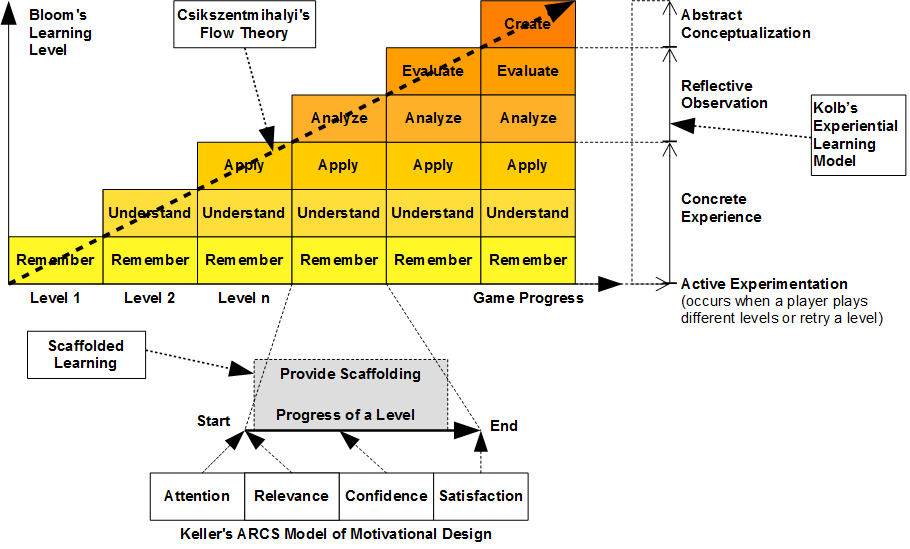
\includegraphics[width=\textwidth]{learning-models}
\caption{Elaborating learning models' contribution to the design of the gamified modeling learning}.
\label{learning-models}
\end{figure}

\begin{figure}[ht]
\centering
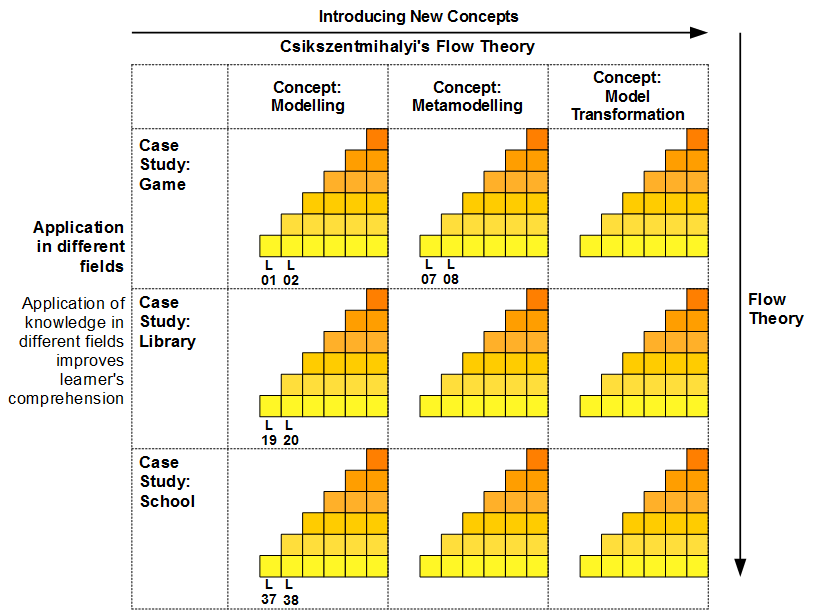
\includegraphics[width=\textwidth]{learning-models2}
\caption{Elaborating learning models' contribution to the design of the gamified modeling learning}.
\label{learning-models2}
\end{figure}

While learners are progressing in the gamification, they are developing their competence. Thus, difficulty has to be kept balanced with their competence, otherwise they will get bored. It is the situation where the theory of Flow can be applied (Figure \ref{learning-models}). To control degree of difficulty, there are three ways we identified so far related to pedagogical approach: a combination of Bloom's activities, the introduction of new concepts, and application in different domains. The order of the levels of each of the three ways has to be arranged properly following the theory of Flow. Concepts that are easier are given earlier than the harder ones, and the difficulty is increased gradually as learners progress. Likewise, Application in the domains that are more familiar with learners should be given first and gradually shifted to the domains that are most unfamiliar (Figure \ref{learning-models}. Combining these three dimensions---types of activities, concepts, and domains---could give us a variety of levels with different degrees of difficulties.

Motivation is an important aspect in the success of learning, and we use Keller's ARCS motivational model to address this aspect \cite{keller2010motivational}. The model provides us in each its components---attention, relevance, confidence, satisfaction---a set of predefined techniques to maintain learners' motivation. In a course of a level of a gamification, there are a start, an end, and learning activities in between (Figure \ref{learning-models}). We could apply the ARCS' techniques to maintain learners' motivation along the course of completing a level. As an example, we could use animation to gain learners' attention, explaining the application of the concept being taught in the currently playing level to give relevance, showing their progress in completing a level to maintain their confidence, and giving them a reward after finishing a level for reward.
 
We apply scaffolding \cite{vygotsky1978mind, wood1976role} to support learners coping challenges (Figure \ref{learning-models}). Throughout finishing a level, scaffolding could be provided in several ways: reducing extensive modelling activities into smaller activity constituents, removing irrelevant activities, providing an almost complete model so they can work on the most relevant activities rather than build the model from scratch, providing help and documentation, and giving some clues of the solutions when they get stuck. This support will be reduced as players progress to maintain the balance between their increasing competence and difficulty.

We also consider applying Kolb's experiential learning model, which is a model that agrees knowledge is constructed through experience and based its model on constructivism \cite{kolb2014experiential}. We select Kolb's model since we perceive that playing a level in a gamification is similar to the learning cycle Kolb proposed; a cycle consists of 4 steps: concrete experience (CE), reflective observation (RO), abstract conceptualisation (AC), and active experimentation (AE). 

We could apply this cycle to frame learners' activities in gaining new knowledge through solving a problem given in a level. For example, the first time players play a new level, at that moment they encounters a concrete experience (CE). Immediately, They attempt to identify and characterise the problem given in that level and recall any knowledge that is relevant to solve the problem (RO). Next, they construct a solution for the problem that they face (AC). After constructing the solution, they apply the solution to the problem (AE), experience the result (CE), and then evaluate whether the solution solves the problem of the level or not (RO). Any gap that appears will update their knowledge. They use their newly updated knowledge to produce a new solution (AC) that could be applied to the same problem at the same level or different problem in other levels (AE). In case that the player already `game Over' and they cannot apply their new solution, AE occurs when they replay the same level or play a similar level.

\begin{table}[ht]
\caption{Requirements derived from learning models (section \ref{Elaborating Design and Learning Models}).}
\label{design-learning-models}
\begin{center}
\begin{tabular}{ p{2cm}p{1cm}p{10cm} } 
\hline
Category & Code & Requirements from Learning Models \\
\hline
\multirow{1}{2cm}{Learning Models} 
& RM01 & Design satisfies Bloom's taxonomy. \\
& RM02 & Design suffices Kolb's experiential learning model. \\ 
& RM03 & Design meets Keller's ARCS motivational model. \\
& RM04 & Design fulfils scaffolded learning. \\
& RM05 & Design complies with the theory of Flow. \\ 
\hline
\end{tabular}
\end{center}
\end{table}

Learning activities in Bloom's taxonomy also correspond to the steps in Kolb's learning cycle \cite{murphy2007prior} and both have been applied together to design instructions in different fields \cite{terry1993kolb, howard1996felder, schatzberg2002applying}. Therefore, we argued that both could be implemented simultaneously; Bloom's taxonomy provides learning activities while Kolb's model addresses learning cycles in the design of our game. To simplify our work, we summarise the elaboration of design and learning models into a list of requirements (Table \ref{design-learning-models}) that will be used in the design and evaluation activities.

\section{Game Design}
\label{Game Design}
Gamification has been successfully for a variety of purposes, but there is very little work on software modelling gamification. We wish to assess whether gamification is beneficial for learners of graphical software modelling languages. We choose graphical modelling languages since they are the common languages used in modelling, whether in academia or industry, and extensively used in Model-Driven Engineering. Standard graphical modelling languages like UML\footnote{\url{http://www.uml.org/}} and BPMN\footnote{\url{http://www.bpmn.org/}}, often used in Model-Driven Engineering, are some of the use-cases.        

Modelling can be expressed in different modelling languages. To ensure the generality of our gamification solution, we plan to support several modelling languages. For each modelling language, we envision the development of a dedicated game containing game elements that will be derived from the Gameful Design Framework \cite{deterding2015lens}. Each game will mimic a graphical modelling tool, and at each level, it will require the learner to graphically construct or adapt a model to satisfy a set of requirements and constraints.

\begin{figure}[ht]
\centering
\frame{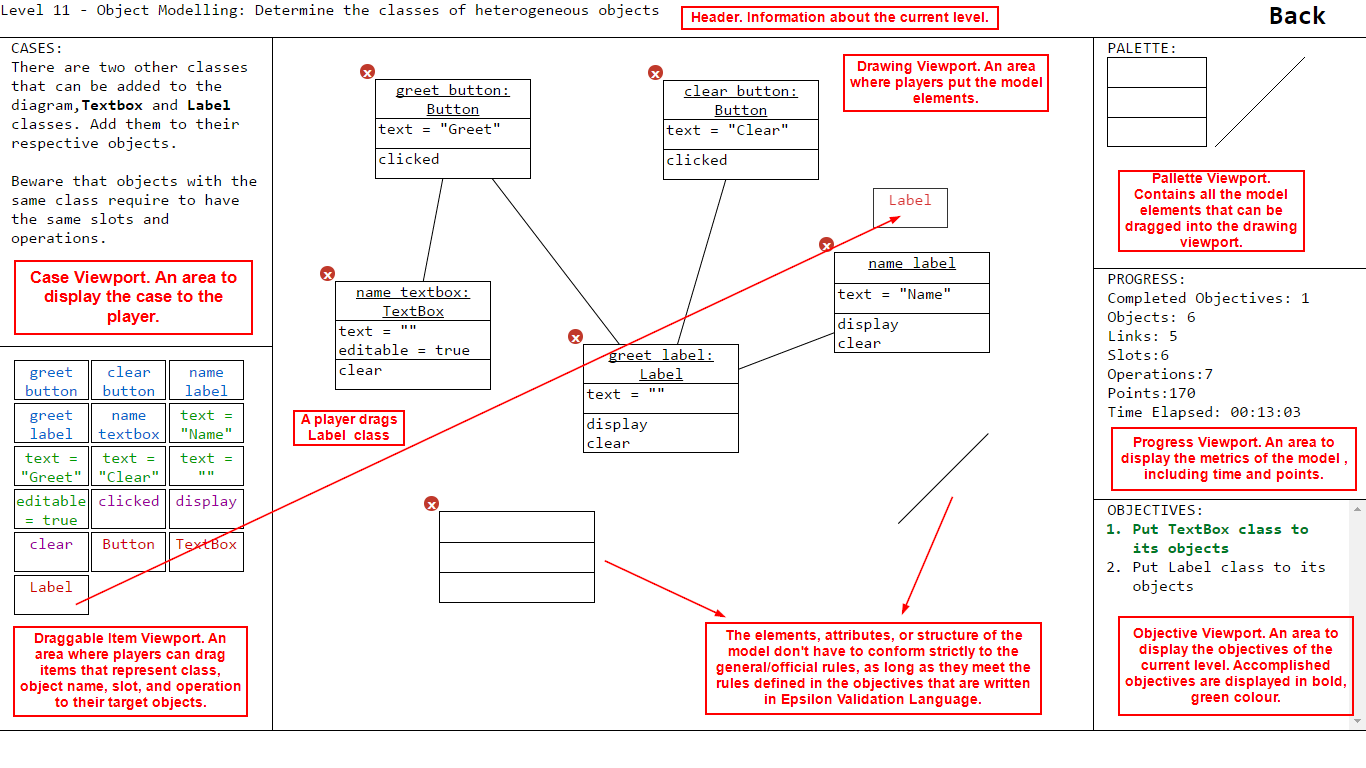
\includegraphics[width=\textwidth]{game-annotated}}
\caption{The display of the generated game.}
\label{fig:001}
\end{figure}

A gamification will have levels of gradually increasing difficulty as well as variety in its challenges, to expose learners to different kinds of domains, models, and diagrams. Tutorials are planned to be embedded into the gamification to help learners familiarise themselves with the control system and the flow of the gamification. 

The gamification will include interim goals and intrinsic rewards to motivate learners. For software modelling, each type of modelling (e.g. object modelling, collaboration, process) will have several stories. A story will represent a specific case study to introduce learners to problems in specific domains. Every story will consist of several levels, and every level will have one or more objectives that a learner needs to accomplish to complete it. A level may also be a continuation of a previous level, giving the learner a sense of step-by-step progress to complete the domain problems. Each story and level will introduce new concepts and link them with previously introduced concepts.

A real-world problem can be very complex and time-consuming to model. Thus, the extraneous activities that are not relevant to the core concepts that are being taught should be removed. As a result, learners will be more focused on the main concepts. Thus, game elements like bite-sized actions (e.g. drag and drop), limited choices (i.e. only limited items can be dragged), and microflows (i.e. put the right element to its right place) will be implemented to facilitate learners in performing the core activities. Likewise, fuzziness will also be used to stimulate learners' creativity since most of the time there is no single correct model for the problem at hand. Attractive design will also be significant to motivate learners to interact with the gamification. Gamification should be able to give instant, noticeable, and actionable feedback to maintain learners' engagement and monitor their progress. Interesting and varied feedback should be designed to appeal to the learners' motives. 

To minimise bias, we plan to experiment with several modelling languages (e.g. BPMN, state-charts, GSN, UML). We also plan to implement the gamification using web technologies so that they are accessible to a wide audience.

The details of the application of Deterding's Gameful Design to our design process are presented in Appendix \ref{Application of Deterding's Gameful Design Steps}. The process also produced storyboards that are the preliminary design of levels and graphical user interface of our game (Appendix \ref{Storyboards}).      

\section{SMLG Design and Generation Framework}
Rather than developing SMLG for each graphical modelling language manually, we plan to follow a model-based approach. In the spirit of Eugenia \cite{kolovos2015eugenia}, we will use metamodel annotations to define the graphical syntaxes of modelling languages and separate models to specify the game elements (constraints,  objectives, levels, etc.) of each game. These models will be then consumed by a model-to-text transformation to produce fully-functional language-specific gamification. Thus, the framework supports software modelling tutors in the design and customisation of the gamification at the high level of abstraction as well as to automatically build the gamification. So far we have implemented a metamodel to specify game elements (flows, levels, challenges, and objectives) and a supporting Eclipse-based graphical editor (Fig. \ref{fig:002}), and a prototype game (Fig. \ref{fig:001}) for object diagrams. 

\begin{figure}[ht]
\centering
\frame{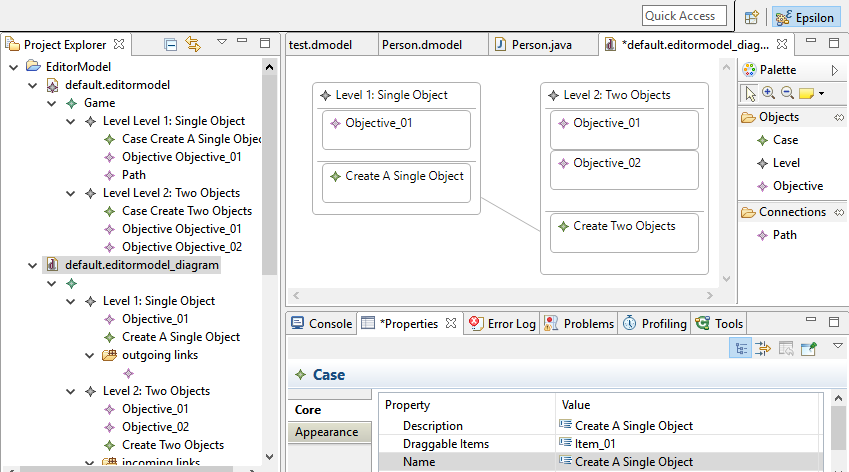
\includegraphics[width=\textwidth]{editor}}
\caption{Graphical editor for the gamification specification DSL.}
\label{fig:002}
\end{figure}

\addcontentsline{toc}{chapter}{Bibliography}
\bibliographystyle{IEEEtran}
\bibliography{references}

\begin{appendices}

\chapter{Research Plan}
\label{Research Plan}

We plan to complete literature study and develop prototype by the end of the first year (2016), and address gamification of modelling and metamodelling in the second year (2017) and third year (2018) respectively. 

\begin {table}[ht]
\caption {Research Timetable} 
\end{table}
\begin{figure}[ht]
\centering
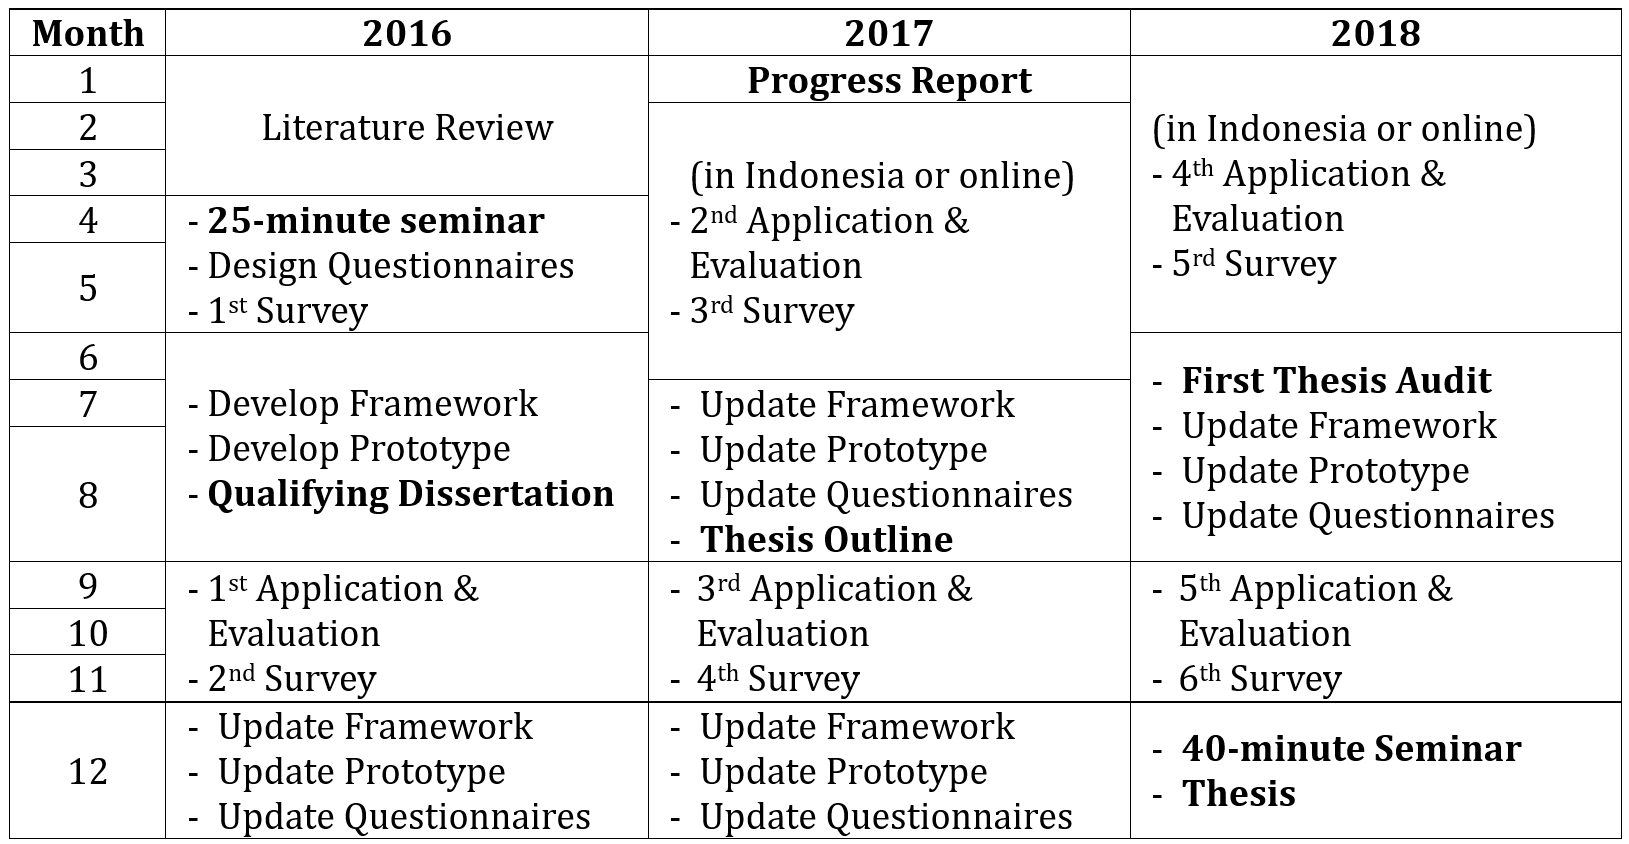
\includegraphics[width=\textwidth]{timetable}
\end{figure}

\chapter{Publications}
We have published papers in the following conferences or journals: 
\begin{enumerate}
 \item A. Yohannis, ``Gamification of software modelling,” in the ACM/IEEE 19th International Conference on Model Driven Engineering Languages and Systems (MODELS 2016) Doctoral Symposium. CEUR, 2016 \cite{Yohannis2016}.
\end{enumerate}

\chapter{Preliminary Survey Data}
\label{chap:Preliminary Survey Data}

\begin{enumerate}
\item \textbf{If you think back to the time when you were just about to start the MODE module, what did you think you would find interesting in Model ­Driven Engineering?}
\begin{itemize}
\item Learning what MDE actually is. Had never heard of it so was intrigued.
\item I thought I would be provided with a high level approach to designing and managing software/critical systems.
\item Learning some tools to create auto­models.
\item Learning about ways of statically verifying that code conformed to a formal model, and using this to detect and automatically correct bugs learning about ways to automatically modify code based on changes made to a model.
\end{itemize}

\item \textbf{What did you find important in Model­ Driven Engineering?}
\begin{itemize}
\item Domain modelling ­ especially metamodels and the whole concept of abstract syntax. Regarding practicalities, the ability to use models to generate code is the most useful, along with creating DSLs.
\item Trying to learn the specific tools to pass the assessment. Not ideal as I wanted more generic
skill sets in this domain I could apply in my career, instead it was too focused on learning some niche features in Epsilon.
\item abstract thinking ­ validate the models ­ linking the model to real­life.
\item The ability to keep a formal model that the code has been verified to conform to throughout
an entire development process Automatic code generation modifcation based on a model.
\end{itemize}

\item \textbf{ Why did you decide to take the Model ­Driven Engineering module?}
\begin{itemize}
\item It was compulsory. I had no choice.
\item Compulsory.
\item well, I feel that everything around me has a certain model. Therefore, I felt learning about. Model­ Driven will increase my knowledge and experience in work. 
\item It seemed like it would be useful to learn a new approach to software engineering and skills that might be valuable in the industry in the future I was interested in generating and transforming code automatically and using a formal model for the structure of the code.
\end{itemize}


\item \textbf{ What would motivate you more to learn Model Driven Engineering?}
\begin{itemize}
\item Seeing the MDE approach being used to do something that would otherwise be much more tedious to do using more conventional means.
\item To see the benefit applied in the real world and how organisations have benefited from it. Then how can use these skills and adapt them to my needs?
\item If we link it to real­life examples, explore more other tools.
\item More use of it in industry More use with languages other than Java and different types of models such as ones that aren't based on UML/EMF.
\end{itemize}

\item \textbf{ Based on the answers that you’ve provided above (No. 1­4), what were the most basic, core underlying motives or needs that make you commit to learning Model­
Driven Engineering?}

\begin{itemize}
\item The ability to think at a higher level of abstraction and understand the concepts which link together a domain ­ especially, for example, programming languages. 
\item Passing the compulsory paper.
\item see some real­life examples and apply different models to see the differences. 
\item Learning skills which would be valuable in the SE industry in the future Learning something which would help with controlling the complexity of a sofware engineering process by making sure that code
conforms to a formally­defined model
\end{itemize}


\item \textbf{ What were the challenges that you found interesting in learning Model­Driven Engineering? Why?}
\begin{itemize}
\item One of the main challenges is in defining the abstract syntax for a DSL along with placing restrictions on its use through a validation language. There's a balance between trying to make the abstract syntax clean and easy to understand and modify vs. preserving the intended semantics.
\item None really, I found the assignment and practicals a tool based grind as opposed to a useful learning opportunity.
\item I sometimes felt that I could not apply all principles in the practicals­ especially on how we think abstract.
\item Working out how to best model a system, which had been defined informally, in EMF and EVL while keeping all its constraints intact and made it easily queryable and transformable was interesting.
\end{itemize}



\item \textbf{How did you manage to overcome these challenges?}
\begin{itemize}
\item By experimenting and going with what makes the most sense. If it is a structural issue with semantics, it is an abstract syntax issue. If it is something more peculiar, it is a validation issue.
\item By grinding through them.
\item I tried to train myself on other examples, but still, I could not link my models to real­life example( as a real project). 
\item The best way to learn this was from experience which was gained by completing all the practicals.
\end{itemize}


\item \textbf{ What were the challenges---the non­interesting challenges---that hindered or demotivated you in learning Model­Driven Engineering? Why?}
\begin{itemize}
\item Learning the Eclipse Modelling Framework, MOF, etc. wasn't fun. The most fun part was learning and use Emfatic with EGL/EGX and EOL in general. However, actually understanding the meta­metamodel and all the ecore stuff seemed pointless. You do not need to understand what EClass, EEnum, EString etc. are. It is just unnecessary detail that's very specific to
Eclipse and not something that you need to know even if you use Epsilon.
\item The focus on the tool as opposed to the high-level concepts and skill sets that would empower me to utilise model-driven engineering in the real world.
\item sometimes the tool itself, you need to re­track all your changes manually, no right answer or a good explanation why this model is good or bad.
\item Problems using eclipse, the shortcomings of EMF, lack of information available on the internet Eclipse is very large, complex and fragile. EMF/ UML ­style models, can be quite restrictive at times when modelling complex relationships, and often requires resorting to EVL. This is annoying because EVL constraints cannot be easily displayed on a diagram and two different languages/systems, EVL and EMF, are being used for similar things. Sometimes two very similar constraints exist where one can be modelled in EMF, and the other can not, and so requires EVL. Although there is a lot of very good documentation available about the languages in Epsilon, there is far less information on the internet about them than what is usually available for popular programming languages and it would be helpful if there was more.
\end{itemize}

\item \textbf{How did you overcome these challenges?}
\begin{itemize}
\item By ignoring them; once I realised they served no purpose for developers.
\item Reading up about the tools and grinding through them.
\item Asking questions, reading some examples in the Epsilon website forum.
\item Eclipse sometimes stops working but does this usually does not prevent the completion of tasks as most problems can be fixed by deleting the workspace directory and starting again, it simply wastes many time Things that could not be expressed in EMF were instead expressed using EVL. The required information about Epsilon could always be found by
asking classmates and asking lecturers, but this would not be possible if using these languages outside the university
\end{itemize}
\end{enumerate}

\chapter{Application of Deterding's Gameful Design Steps}
\label{Application of Deterding's Gameful Design Steps}


\section{Strategy}
\subsection{Define Target Outcome and Metrics}
\subsubsection{Outcome}
\begin{itemize}
\item Students that use the gamified learning perform better than traditional ones in software modelling.
\end{itemize}

\subsubsection{Metrics}
\begin{itemize}
\item Scores that they get from solving given software modelling problems.
\item Subjective opinions that learning through the gamified systems is better than the traditional ones. 
\item Model metrics of the models that they produce.
\end{itemize}

\subsection{Define Target Users, Context, Activities}
\subsubsection{Users}
Computer Science Undergraduate Students with some knowledge of object-orientation, ideally from both programming and design, and a good understanding of software engineering
\subsubsection{Context}
One term of software modelling course (Time) and in the context of university software modelling course (Place)
\subsubsection{Activities}
Modelling, metamodelling, and model management

\subsection{Identify Constraints and Requirements}
\subsubsection{Laws and regulations}
\begin{itemize}
\item Privacy regulation.
\end{itemize}
\subsubsection{Scope (time, budget, personnel)}
\begin{itemize}
\item Time. One term of software modelling.
\item People. Student of software modelling-related courses.
\item Budget. Available research budget.
\end{itemize}
\subsubsection{Technological requirements}
\begin{itemize}
\item Notebooks, computer desktops.
\item Internet connection.
\end{itemize}
\subsubsection{Others}
\begin{itemize}
\item Align with the existing learning models and software modelling teaching best practices.
\end{itemize}

\section{Research}
\subsection{Translate Users Activities into Behaviour Chains}
\subsubsection{Modelling}
\begin{itemize}
\item Real-world problems are given using textual description (or videos, interviews, images, etc.) 
\item Perform abstraction/identify relevant concepts (objects, values, attributes, and operations) according to the requirements 
\item Translate them into classes and relationships
\item Construct the model in the form of diagrams that represent the classes and relationships in different views (different diagrams)
\item Evaluate the models
\end{itemize}

\subsubsection{Meta-Modelling}
\begin{itemize}
\item Models are given using textual description (or videos, interviews, images, figures, etc.) 
\item Perform abstraction/identify relevant concepts (classes, relationships, attributes) of the models
\item Translate them into metamodel classes
\item Construct metamodel diagrams that represent the metamodel
\item Evaluate the metamodel
\end{itemize}

\subsubsection{Model Management}
\begin{itemize}
\item Problems are given using textual description (or videos, interviews, images, figures, etc.) 
\item Identify goals and constraints
\item Determine the model management operations:
Validation
\item Transformation (model-to-model, text-to-model, model-to-text)
Etc.
\item Refine the operations into more detail steps
\item Test
\item Execute
\end{itemize}

\subsection{Identify User Needs, Motivations, challenges}
\subsubsection{User needs}
\begin{itemize}
\item Master the software modelling.
\end{itemize}
\subsubsection{Motivations}
\begin{itemize}
\item Has competency in software modelling (Ability to solve problems and ability to produce artefacts or concrete products).
\item Fun, challenging.
\item Understanding the importance and advantages of software modelling.
\end{itemize}
\subsubsection{challenges}
\begin{itemize}
\item No fun, the presentation of software modelling is not interesting.
\item Abstraction is difficult, choosing the most relevant elements according to the requirements.
\item Heavy cognitive loads dealing with abstract concepts.
\end{itemize}

\subsection{Determine Gameful Design Fit}
\begin{itemize}
\item Does the activity connect to an actual user need? \textbf{Yes}
\item Is lacking motivation a central issue or opportunity (and not, e.g., poor usability)? \textbf{Both}
\item Does the target activity involve an inherent challenge with a learnable skill? \textbf{Yes}
\item Is affording experiences of competence the most effective and efficient way of improving motivation (and not, e.g., defusing fears)? \textbf{Yes}
\end{itemize}

\section{Synthesis}
\subsection{Formulate Activity, Challenge, Motivation  Triplets for Opportune Activities or Behaviours}

\subsubsection{What motivations energize and direct the activity?}
Software modelling mastery: solving problems and build abstract/concrete artefacts
\subsubsection{What challenges are inherent in the activity?}
\begin{itemize}
\item Abstraction: determine the most relevant objects and relationships between them
\item Diagramming: translate the resulting model into diagram
\item Algorithmic operation: much like programming but for model management
\end{itemize}
\subsubsection{What challenges can be removed through automation or improving usability?} 
\begin{itemize}
\item Simplify the real-world scenario to identify relevant objects
\item Simplify the diagramming processes
\item Simplify the algorithmic operations
\end{itemize}
\subsubsection{What challenges remain that the user can learn to get better at?}
Abstraction, diagramming, algorithmic operation
\subsubsection{What are the activities, challenges, and motives?}
\begin{itemize}
\item Activity: Construct model 
\item Challenge: abstraction, diagramming, algorithmic operation
\item Motive: fear to make mistakes (-), solving problems (+), create artefacts (+)
\end{itemize}

\section{Ideation}
\subsection{Brainstorming Ideas using Innovation Stems}
\subsubsection{Challenge lenses}
Onboarding, scaffolded challenge, varied challenge 
\subsubsection{Goal and motivation lenses}
Interim goals, viral calls to action, next base action, intrinsic rewards, secrets, templates, traces of others
\subsubsection{Action and object lenses}
Bite sized actions, interesting choices, limited choices, micro-flow, small pieces loosely joined, expressive objects, underdetermination, sensual objects
\subsubsection{Feedback lenses}
Immediate, juicy, actionable, appeal to motives, glanceable, varied, surprising, graspable progress.

\subsubsection{Example}
\begin{itemize}
\item Scaffolded challenge lens and Mastery motivation
How might we spark a sense of mastery in abstraction,  diagramming, and model operation?
\item How might we use scaffolded challenge to make the abstraction, diagramming, and model operation more enjoyable?
\item How might we spark a sense of mastery with scaffolded challenge?
\item How might we alleviate fear of making mistakes with scaffolded challenges?
\end{itemize}

\subsection{Prioritise Ideas}
Only one idea created so far. Learners are given a scaffolded series of problems to which they can exercise modelling, metamodelling, and model management. Motivating feedbacks to achieve mastery are integrated as well.

\section{Iterative Prototyping}
Prototyping is still on going work.


\chapter{Storyboard: Object Diagram}
\label{Storyboards}
\begin{itemize}
\item Objects
	\begin{itemize}
	\item Create single object (Level 01)
	\item Create two objects (Level 02)
	\item Create multiple objects (Level 03)
	\end{itemize}
\item Links (Relationships)
	\begin{itemize}
	\item Create single link (Level 04)
	\item Create multiple links (Level 05)
	\end{itemize}
\item Slots (Attributes)
	\begin{itemize}
	\item Determine a slot and its value (Level 06)
	\item Determine slots and their values (Level 07)
	\end{itemize}
\item Operations/Methods
	\begin{itemize}
	\item Determine operation (Level 08)
	\item Determine multiple (Level 09) operations
	\end{itemize}
\item Class of Objects
	\begin{itemize}
	\item Determine the class of homogeneous objects (Level 10)
	\item Determine different classes of heterogeneous objects (Level 11)
	\end{itemize}
\item Case Studies
	\begin{itemize}
	\item Reconstruct the model from the beginning (Level 12)
	\item Apply the skills on different/similar problem (Level 13)
	\end{itemize}
\end{itemize}

\begin{figure}[ht]
    \centering
    \subfloat[Level 01]{{ \frame{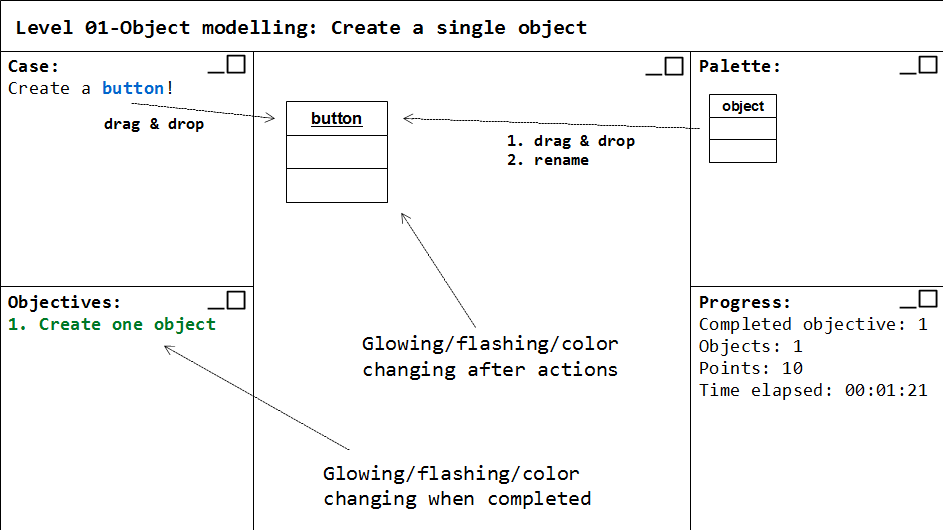
\includegraphics[width=7.16cm]{storyboard01}} }}
    \hspace{0cm}
    \subfloat[Level 02]{{ \frame{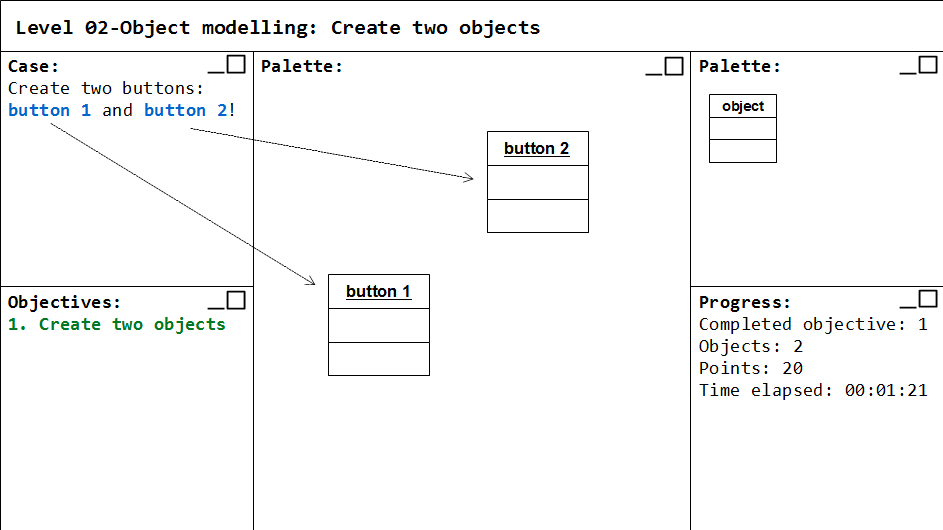
\includegraphics[width=7.16cm]{storyboard02}} }}
    \\
    \subfloat[Level 03]{{ \frame{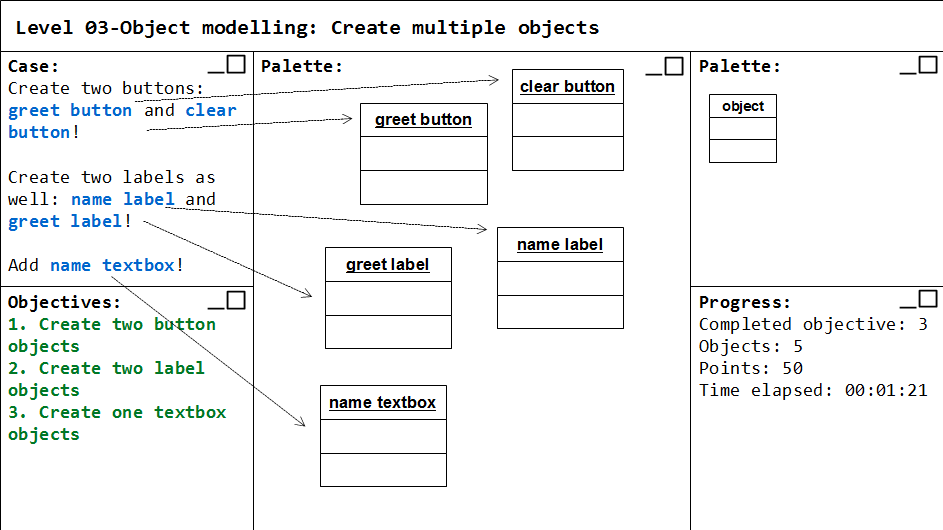
\includegraphics[width=7.16cm]{storyboard03}} }}
    \hspace{0cm}
    \subfloat[Level 04]{{ \frame{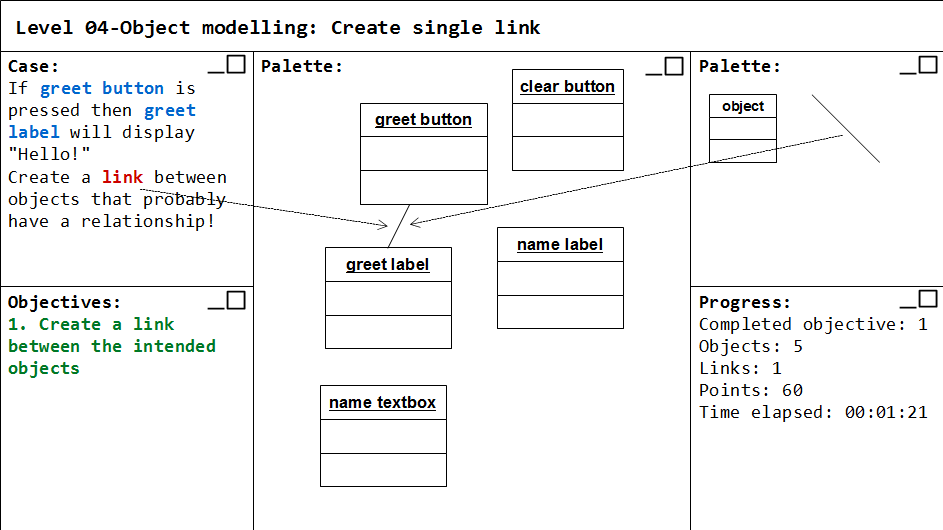
\includegraphics[width=7.16cm]{storyboard04}} }}
    \\
    \subfloat[Level 05]{{ \frame{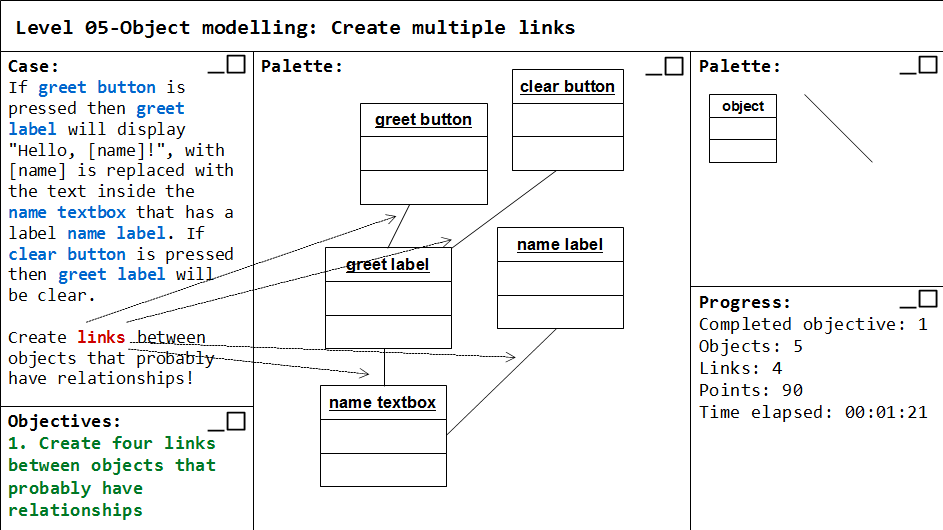
\includegraphics[width=7.16cm]{storyboard05}} }}
    \hspace{0cm}
    \subfloat[Level 06]{{ \frame{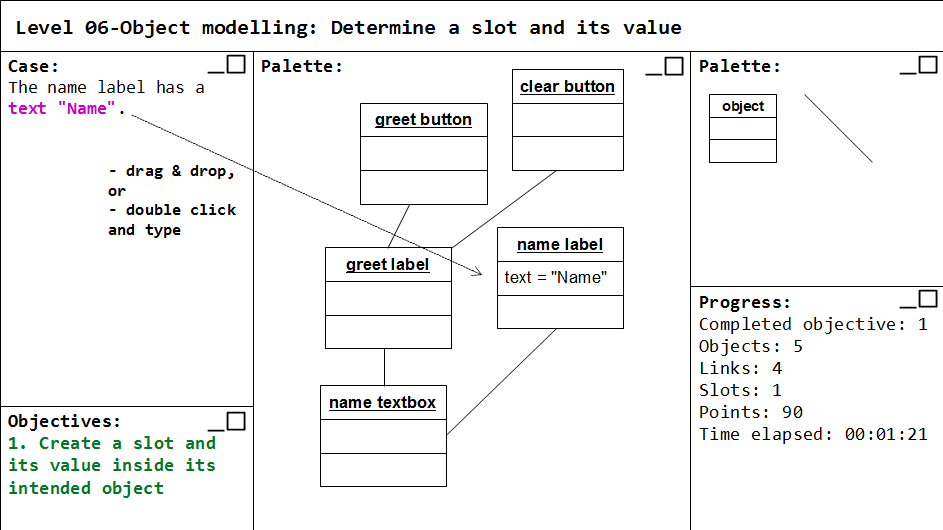
\includegraphics[width=7.16cm]{storyboard06}} }}
    
    
    
    \caption{Storyboard of Gamification of Object Diagram (part 1).}
    \label{storyboard-1}
\end{figure}


\begin{figure}[ht]
    \centering
    \subfloat[Level 07]{{ \frame{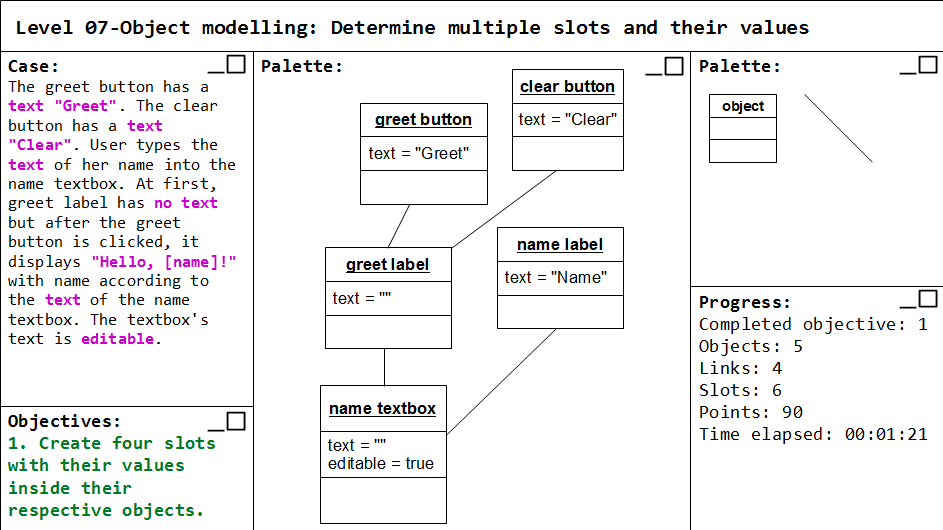
\includegraphics[width=7.16cm]{storyboard07}} }}
    \hspace{0cm}
    \subfloat[Level 08]{{ \frame{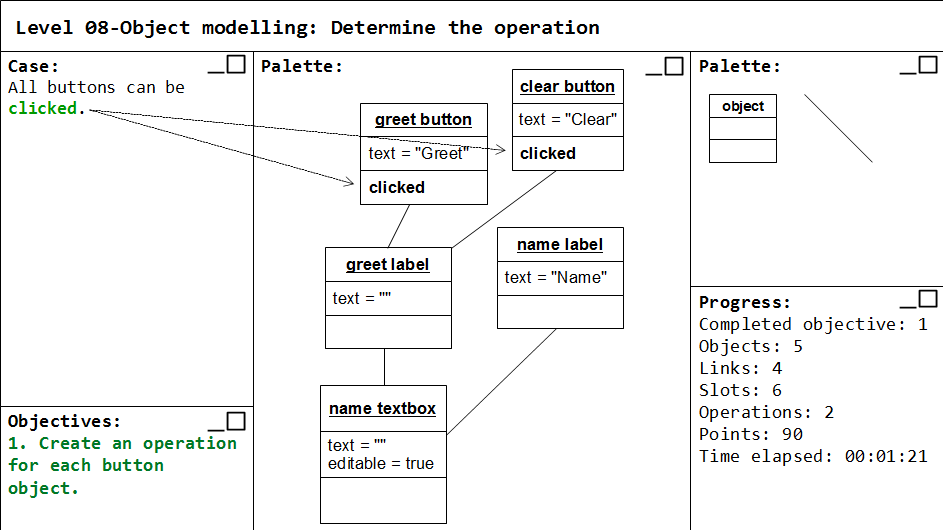
\includegraphics[width=7.16cm]{storyboard08}} }}
    \\
    \subfloat[Level 09]{{ \frame{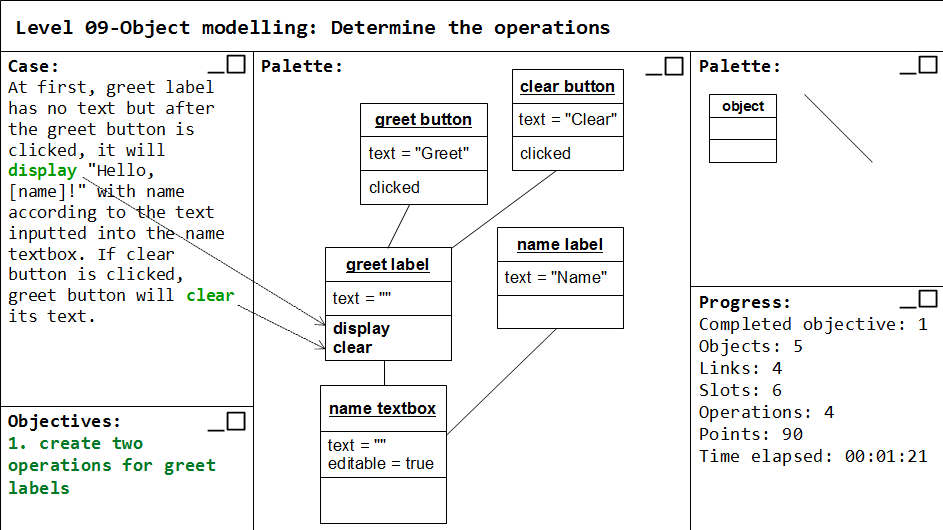
\includegraphics[width=7.16cm]{storyboard09}} }}
    \hspace{0cm}
    \subfloat[Level 10]{{ \frame{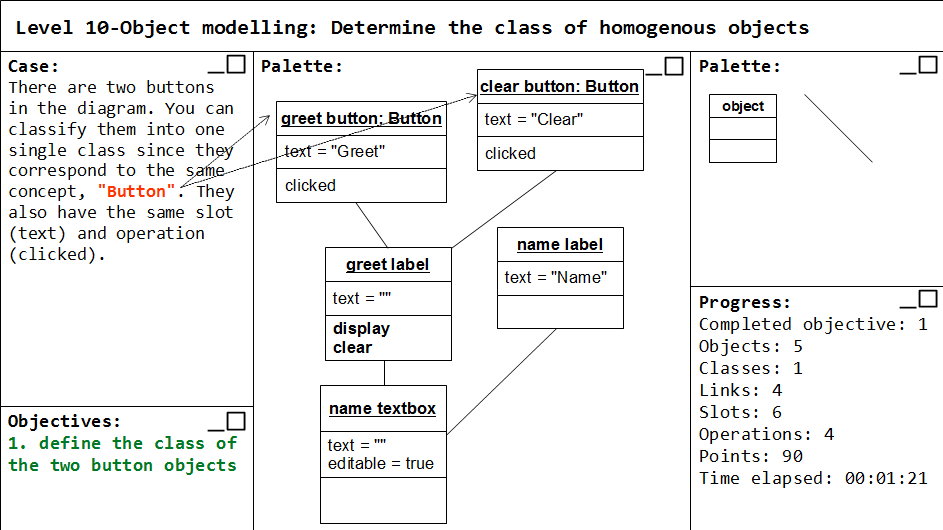
\includegraphics[width=7.16cm]{storyboard10}} }}
    \\
    \subfloat[Level 11]{{ \frame{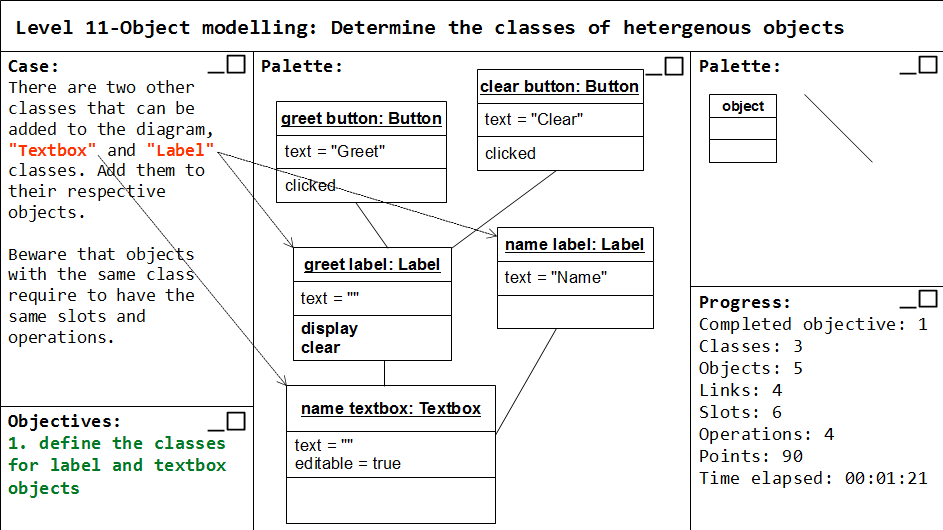
\includegraphics[width=7.16cm]{storyboard11}} }}
    \hspace{0cm}
    \subfloat[Level 12]{{ \frame{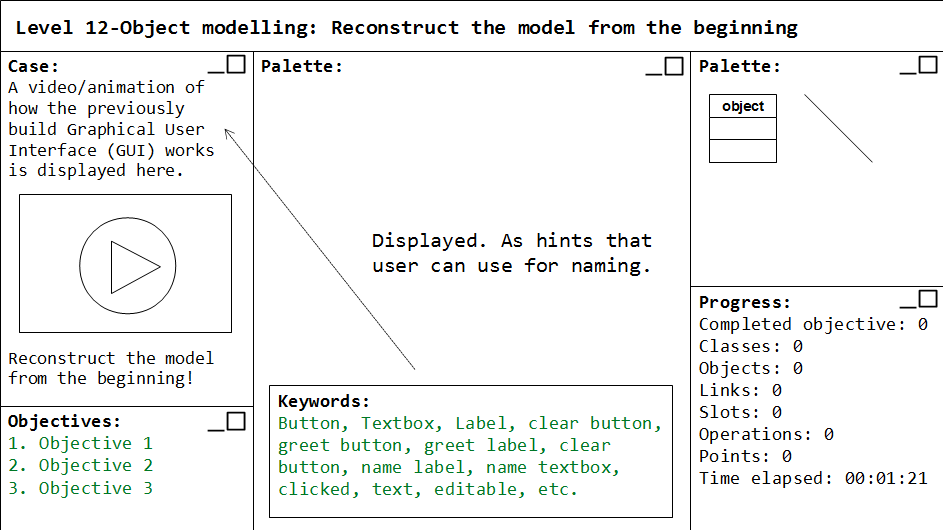
\includegraphics[width=7.16cm]{storyboard12}} }}
\caption{Storyboard of Gamification of Object Diagram (part 2).}
    \label{storyboard-2}
\end{figure}


\end{appendices}

\end{document}




